% Options for packages loaded elsewhere
\PassOptionsToPackage{unicode}{hyperref}
\PassOptionsToPackage{hyphens}{url}
%
\documentclass[
]{article}
\usepackage{amsmath,amssymb}
\usepackage{lmodern}
\usepackage{iftex}
\ifPDFTeX
  \usepackage[T1]{fontenc}
  \usepackage[utf8]{inputenc}
  \usepackage{textcomp} % provide euro and other symbols
\else % if luatex or xetex
  \usepackage{unicode-math}
  \defaultfontfeatures{Scale=MatchLowercase}
  \defaultfontfeatures[\rmfamily]{Ligatures=TeX,Scale=1}
\fi
% Use upquote if available, for straight quotes in verbatim environments
\IfFileExists{upquote.sty}{\usepackage{upquote}}{}
\IfFileExists{microtype.sty}{% use microtype if available
  \usepackage[]{microtype}
  \UseMicrotypeSet[protrusion]{basicmath} % disable protrusion for tt fonts
}{}
\makeatletter
\@ifundefined{KOMAClassName}{% if non-KOMA class
  \IfFileExists{parskip.sty}{%
    \usepackage{parskip}
  }{% else
    \setlength{\parindent}{0pt}
    \setlength{\parskip}{6pt plus 2pt minus 1pt}}
}{% if KOMA class
  \KOMAoptions{parskip=half}}
\makeatother
\usepackage{xcolor}
\usepackage[margin=1in]{geometry}
\usepackage{color}
\usepackage{fancyvrb}
\newcommand{\VerbBar}{|}
\newcommand{\VERB}{\Verb[commandchars=\\\{\}]}
\DefineVerbatimEnvironment{Highlighting}{Verbatim}{commandchars=\\\{\}}
% Add ',fontsize=\small' for more characters per line
\usepackage{framed}
\definecolor{shadecolor}{RGB}{248,248,248}
\newenvironment{Shaded}{\begin{snugshade}}{\end{snugshade}}
\newcommand{\AlertTok}[1]{\textcolor[rgb]{0.94,0.16,0.16}{#1}}
\newcommand{\AnnotationTok}[1]{\textcolor[rgb]{0.56,0.35,0.01}{\textbf{\textit{#1}}}}
\newcommand{\AttributeTok}[1]{\textcolor[rgb]{0.77,0.63,0.00}{#1}}
\newcommand{\BaseNTok}[1]{\textcolor[rgb]{0.00,0.00,0.81}{#1}}
\newcommand{\BuiltInTok}[1]{#1}
\newcommand{\CharTok}[1]{\textcolor[rgb]{0.31,0.60,0.02}{#1}}
\newcommand{\CommentTok}[1]{\textcolor[rgb]{0.56,0.35,0.01}{\textit{#1}}}
\newcommand{\CommentVarTok}[1]{\textcolor[rgb]{0.56,0.35,0.01}{\textbf{\textit{#1}}}}
\newcommand{\ConstantTok}[1]{\textcolor[rgb]{0.00,0.00,0.00}{#1}}
\newcommand{\ControlFlowTok}[1]{\textcolor[rgb]{0.13,0.29,0.53}{\textbf{#1}}}
\newcommand{\DataTypeTok}[1]{\textcolor[rgb]{0.13,0.29,0.53}{#1}}
\newcommand{\DecValTok}[1]{\textcolor[rgb]{0.00,0.00,0.81}{#1}}
\newcommand{\DocumentationTok}[1]{\textcolor[rgb]{0.56,0.35,0.01}{\textbf{\textit{#1}}}}
\newcommand{\ErrorTok}[1]{\textcolor[rgb]{0.64,0.00,0.00}{\textbf{#1}}}
\newcommand{\ExtensionTok}[1]{#1}
\newcommand{\FloatTok}[1]{\textcolor[rgb]{0.00,0.00,0.81}{#1}}
\newcommand{\FunctionTok}[1]{\textcolor[rgb]{0.00,0.00,0.00}{#1}}
\newcommand{\ImportTok}[1]{#1}
\newcommand{\InformationTok}[1]{\textcolor[rgb]{0.56,0.35,0.01}{\textbf{\textit{#1}}}}
\newcommand{\KeywordTok}[1]{\textcolor[rgb]{0.13,0.29,0.53}{\textbf{#1}}}
\newcommand{\NormalTok}[1]{#1}
\newcommand{\OperatorTok}[1]{\textcolor[rgb]{0.81,0.36,0.00}{\textbf{#1}}}
\newcommand{\OtherTok}[1]{\textcolor[rgb]{0.56,0.35,0.01}{#1}}
\newcommand{\PreprocessorTok}[1]{\textcolor[rgb]{0.56,0.35,0.01}{\textit{#1}}}
\newcommand{\RegionMarkerTok}[1]{#1}
\newcommand{\SpecialCharTok}[1]{\textcolor[rgb]{0.00,0.00,0.00}{#1}}
\newcommand{\SpecialStringTok}[1]{\textcolor[rgb]{0.31,0.60,0.02}{#1}}
\newcommand{\StringTok}[1]{\textcolor[rgb]{0.31,0.60,0.02}{#1}}
\newcommand{\VariableTok}[1]{\textcolor[rgb]{0.00,0.00,0.00}{#1}}
\newcommand{\VerbatimStringTok}[1]{\textcolor[rgb]{0.31,0.60,0.02}{#1}}
\newcommand{\WarningTok}[1]{\textcolor[rgb]{0.56,0.35,0.01}{\textbf{\textit{#1}}}}
\usepackage{graphicx}
\makeatletter
\def\maxwidth{\ifdim\Gin@nat@width>\linewidth\linewidth\else\Gin@nat@width\fi}
\def\maxheight{\ifdim\Gin@nat@height>\textheight\textheight\else\Gin@nat@height\fi}
\makeatother
% Scale images if necessary, so that they will not overflow the page
% margins by default, and it is still possible to overwrite the defaults
% using explicit options in \includegraphics[width, height, ...]{}
\setkeys{Gin}{width=\maxwidth,height=\maxheight,keepaspectratio}
% Set default figure placement to htbp
\makeatletter
\def\fps@figure{htbp}
\makeatother
\setlength{\emergencystretch}{3em} % prevent overfull lines
\providecommand{\tightlist}{%
  \setlength{\itemsep}{0pt}\setlength{\parskip}{0pt}}
\setcounter{secnumdepth}{5}
\ifLuaTeX
  \usepackage{selnolig}  % disable illegal ligatures
\fi
\IfFileExists{bookmark.sty}{\usepackage{bookmark}}{\usepackage{hyperref}}
\IfFileExists{xurl.sty}{\usepackage{xurl}}{} % add URL line breaks if available
\urlstyle{same} % disable monospaced font for URLs
\hypersetup{
  pdftitle={Introductie},
  pdfauthor={Lieven Clement},
  hidelinks,
  pdfcreator={LaTeX via pandoc}}

\title{Introductie}
\author{Lieven Clement}
\date{statOmics, Ghent University (\url{https://statomics.github.io})}

\begin{document}
\maketitle

{
\setcounter{tocdepth}{2}
\tableofcontents
}
\hypertarget{longvolume-en-rokerstatus}{%
\section{Longvolume en rokerstatus}\label{longvolume-en-rokerstatus}}

\begin{itemize}
\tightlist
\item
  Onderzoekers willen de impact van roken onderzoeken op longcapaciteit
  bij schoolgaande kinderen en adolescenten.
\item
  Ze meten hierbij de longcapaciteit (in l) bij rokende en niet-rokende
  leerlingen (forced expiratory volume).
\end{itemize}

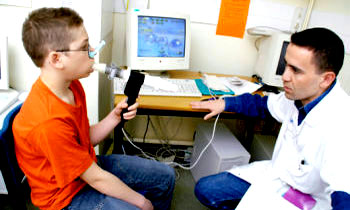
\includegraphics{https://raw.githubusercontent.com/statOmics/biostatistics21/master/figs/fevMeasurement.jpg}

\hypertarget{importeer-data}{%
\subsection{Importeer data}\label{importeer-data}}

\begin{Shaded}
\begin{Highlighting}[]
\FunctionTok{library}\NormalTok{(tidyverse)}
\NormalTok{fev }\OtherTok{\textless{}{-}} \FunctionTok{read\_tsv}\NormalTok{(}\StringTok{"https://raw.githubusercontent.com/GTPB/PSLS20/master/data/fev.txt"}\NormalTok{)}
\end{Highlighting}
\end{Shaded}

\begin{verbatim}
## Rows: 606 Columns: 5
## -- Column specification --------------------------------------------------------
## Delimiter: "\t"
## chr (1): gender
## dbl (4): age, fev, height, smoking
## 
## i Use `spec()` to retrieve the full column specification for this data.
## i Specify the column types or set `show_col_types = FALSE` to quiet this message.
\end{verbatim}

\begin{Shaded}
\begin{Highlighting}[]
\FunctionTok{head}\NormalTok{(fev)}
\end{Highlighting}
\end{Shaded}

\begin{verbatim}
## # A tibble: 6 x 5
##     age   fev height gender smoking
##   <dbl> <dbl>  <dbl> <chr>    <dbl>
## 1     9  1.71   57   f            0
## 2     8  1.72   67.5 f            0
## 3     7  1.72   54.5 f            0
## 4     9  1.56   53   m            0
## 5     9  1.90   57   m            0
## 6     8  2.34   61   f            0
\end{verbatim}

\hypertarget{data-manipulatie}{%
\subsection{Data manipulatie}\label{data-manipulatie}}

\begin{enumerate}
\def\labelenumi{\arabic{enumi}.}
\tightlist
\item
  \texttt{gender} and \texttt{smoking} kunnen beter worden omgezet naar
  factor variabelen
\item
  De \texttt{height} variabele is in inches dus deze zetten we om in cm.
\end{enumerate}

\begin{Shaded}
\begin{Highlighting}[]
\NormalTok{fev }\OtherTok{\textless{}{-}}\NormalTok{ fev }\SpecialCharTok{\%\textgreater{}\%}
  \FunctionTok{mutate}\NormalTok{(}\AttributeTok{gender =} \FunctionTok{as.factor}\NormalTok{(gender)) }\SpecialCharTok{\%\textgreater{}\%}
  \FunctionTok{mutate}\NormalTok{(}\AttributeTok{smoking =} \FunctionTok{as.factor}\NormalTok{(smoking)) }\SpecialCharTok{\%\textgreater{}\%}
  \FunctionTok{mutate}\NormalTok{(}\AttributeTok{height\_cm =}\NormalTok{ height}\SpecialCharTok{*}\FloatTok{2.54}\NormalTok{)}
\FunctionTok{head}\NormalTok{(fev)}
\end{Highlighting}
\end{Shaded}

\begin{verbatim}
## # A tibble: 6 x 6
##     age   fev height gender smoking height_cm
##   <dbl> <dbl>  <dbl> <fct>  <fct>       <dbl>
## 1     9  1.71   57   f      0            145.
## 2     8  1.72   67.5 f      0            171.
## 3     7  1.72   54.5 f      0            138.
## 4     9  1.56   53   m      0            135.
## 5     9  1.90   57   m      0            145.
## 6     8  2.34   61   f      0            155.
\end{verbatim}

\hypertarget{enkele-concepten}{%
\subsection{Enkele Concepten}\label{enkele-concepten}}

\begin{itemize}
\item
  In een \textbf{experimentele studie} gaat een onderzoeker de
  \textbf{behandeling} \textbf{at random} toewijzen aan de
  \textbf{experimentele eenheden} en observeert hij/zij het effect van
  de \textbf{behandeling} bij de experimentele eenheden door het meten
  van één of meerdere \textbf{reponse variabelen}.
\item
  Een \textbf{experimentele eenheid} (experimental unit) is de eenheid
  (subject, plant, pot, proefdier) dat at random aan de behandeling
  wordt toegewezen. \textbf{Experimentele eenheden in fev example?}
\item
  Een \textbf{response variabele} is a karakteristiek van de
  experimentele eenheid die wordt gemeten en geanalyseerd om het effect
  van de behandeling na te gaan. \textbf{Response variable in fev
  example?}
\item
  Een \textbf{observationele eenheid} is de eenheid waarop de response
  variabele wordt gemeten. Veelal is er een één-op-één overeenkomst
  tussen experimentele en observationele eenheden. Maar dat is niet
  altijd zo: b.v. pseudoreplicatie zoals wanneer men technische
  herhalingen heeft voor elke gemeten karakteristiek bij een subject.
  \textbf{Observationele eenheid in fev voorbeeld?}
\item
  Een \textbf{factor} is een verklarende variabele die twee of meer
  niveaus aan kan nemen. Voorbeelden in de fev studie?
\end{itemize}

\begin{center}\rule{0.5\linewidth}{0.5pt}\end{center}

\begin{center}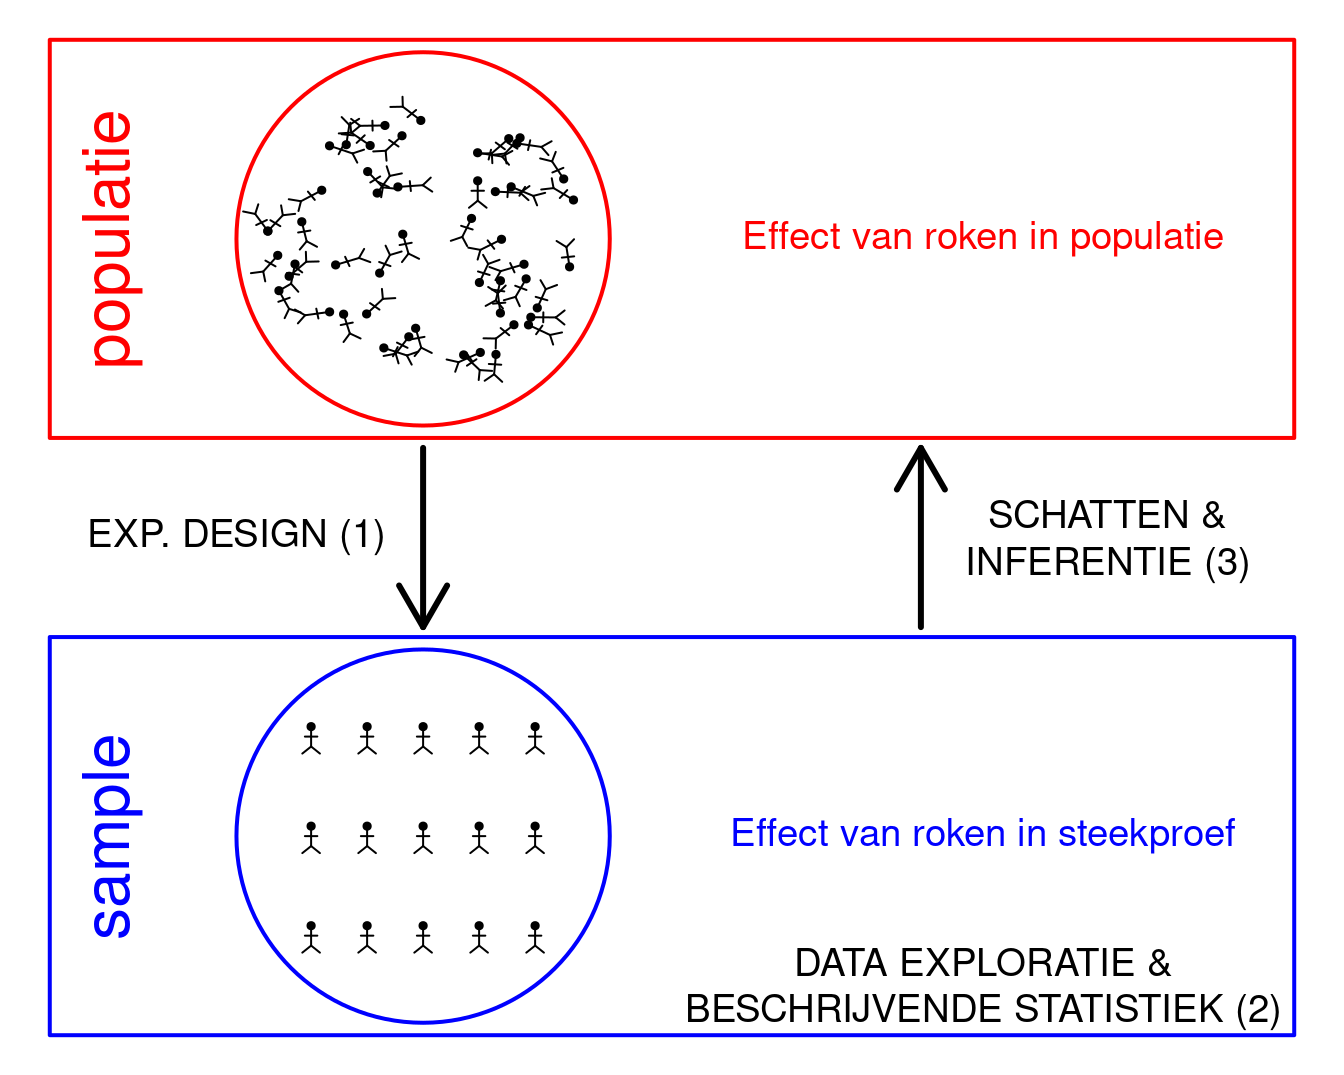
\includegraphics{introduction_files/figure-latex/pop2Samp2Pop-1} \end{center}

\begin{itemize}
\tightlist
\item
  Populatie?
\end{itemize}

\begin{center}\rule{0.5\linewidth}{0.5pt}\end{center}

\hypertarget{data-exploratie}{%
\subsection{Data Exploratie}\label{data-exploratie}}

\hypertarget{summary-statistics}{%
\subsubsection{Summary statistics}\label{summary-statistics}}

\begin{Shaded}
\begin{Highlighting}[]
\NormalTok{fevSum }\OtherTok{\textless{}{-}}\NormalTok{ fev }\SpecialCharTok{\%\textgreater{}\%}
  \FunctionTok{group\_by}\NormalTok{(smoking) }\SpecialCharTok{\%\textgreater{}\%}
  \FunctionTok{summarize\_at}\NormalTok{(}\StringTok{"fev"}\NormalTok{, }
               \FunctionTok{list}\NormalTok{(}\AttributeTok{mean =}\NormalTok{ mean,}
                    \AttributeTok{sd =}\NormalTok{ sd,}
                    \AttributeTok{n =}\NormalTok{ length)}
\NormalTok{                ) }\SpecialCharTok{\%\textgreater{}\%}
  \FunctionTok{mutate}\NormalTok{(}\AttributeTok{se =}\NormalTok{ sd}\SpecialCharTok{/}\FunctionTok{sqrt}\NormalTok{(n))}
\NormalTok{fevSum}
\end{Highlighting}
\end{Shaded}

\begin{verbatim}
## # A tibble: 2 x 5
##   smoking  mean    sd     n     se
##   <fct>   <dbl> <dbl> <int>  <dbl>
## 1 0        2.63 0.816   545 0.0350
## 2 1        3.24 0.752    61 0.0963
\end{verbatim}

\begin{itemize}
\tightlist
\item
  Let op dat deze code niet werkt als er ontbrekende data zijn.
\item
  In dat geval gebruik je onderstaande code
\end{itemize}

\begin{Shaded}
\begin{Highlighting}[]
\NormalTok{fevSum }\OtherTok{\textless{}{-}}\NormalTok{ fev }\SpecialCharTok{\%\textgreater{}\%}
  \FunctionTok{group\_by}\NormalTok{(smoking) }\SpecialCharTok{\%\textgreater{}\%}
    \FunctionTok{summarize\_at}\NormalTok{(}\StringTok{"fev"}\NormalTok{,}\FunctionTok{list}\NormalTok{(}\AttributeTok{mean=}\SpecialCharTok{\textasciitilde{}}\FunctionTok{mean}\NormalTok{(.,}\AttributeTok{na.rm=}\ConstantTok{TRUE}\NormalTok{),}
                    \AttributeTok{sd=}\SpecialCharTok{\textasciitilde{}}\FunctionTok{sd}\NormalTok{(.,}\AttributeTok{na.rm=}\ConstantTok{TRUE}\NormalTok{),}
                    \AttributeTok{n=}\ControlFlowTok{function}\NormalTok{(x) x}\SpecialCharTok{\%\textgreater{}\%}\NormalTok{is.na}\SpecialCharTok{\%\textgreater{}\%}\StringTok{\textasciigrave{}}\AttributeTok{!}\StringTok{\textasciigrave{}}\SpecialCharTok{\%\textgreater{}\%}\NormalTok{sum)) }\SpecialCharTok{\%\textgreater{}\%}
  \FunctionTok{mutate}\NormalTok{(}\AttributeTok{se=}\NormalTok{sd}\SpecialCharTok{/}\FunctionTok{sqrt}\NormalTok{(n))}
\NormalTok{fevSum}
\end{Highlighting}
\end{Shaded}

\begin{verbatim}
## # A tibble: 2 x 5
##   smoking  mean    sd     n     se
##   <fct>   <dbl> <dbl> <int>  <dbl>
## 1 0        2.63 0.816   545 0.0350
## 2 1        3.24 0.752    61 0.0963
\end{verbatim}

\hypertarget{visualisatie}{%
\subsection{Visualisatie}\label{visualisatie}}

\begin{Shaded}
\begin{Highlighting}[]
\NormalTok{fev }\SpecialCharTok{\%\textgreater{}\%}
  \FunctionTok{ggplot}\NormalTok{(}\FunctionTok{aes}\NormalTok{(}\AttributeTok{x =}\NormalTok{ smoking, }\AttributeTok{y =}\NormalTok{ fev)) }\SpecialCharTok{+}
  \FunctionTok{geom\_boxplot}\NormalTok{(}\AttributeTok{outlier.shape =} \ConstantTok{NA}\NormalTok{) }\SpecialCharTok{+}
  \FunctionTok{geom\_jitter}\NormalTok{(}\AttributeTok{alpha =}\NormalTok{ .}\DecValTok{2}\NormalTok{)}
\end{Highlighting}
\end{Shaded}

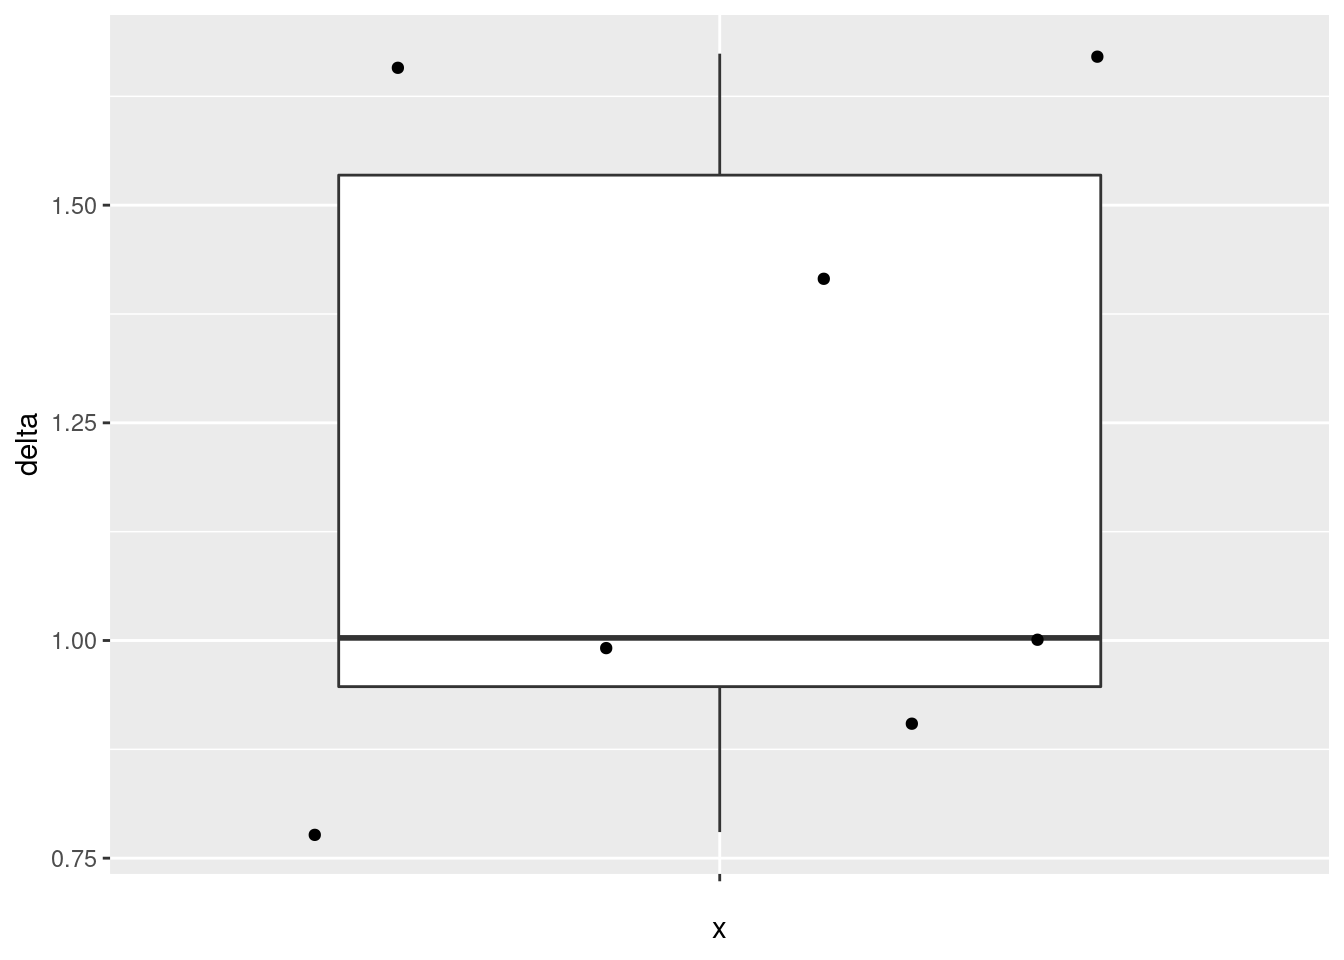
\includegraphics{introduction_files/figure-latex/unnamed-chunk-7-1.pdf}

\begin{itemize}
\tightlist
\item
  Effect grootte?
\end{itemize}

We kunnen de plots ook als objecten opslaan voor later gebruik!

\begin{Shaded}
\begin{Highlighting}[]
\NormalTok{p1 }\OtherTok{\textless{}{-}}\NormalTok{ fev }\SpecialCharTok{\%\textgreater{}\%}
  \FunctionTok{ggplot}\NormalTok{(}\FunctionTok{aes}\NormalTok{(}\AttributeTok{x=}\NormalTok{smoking,}\AttributeTok{y=}\NormalTok{fev)) }\SpecialCharTok{+}
  \FunctionTok{geom\_boxplot}\NormalTok{(}\AttributeTok{outlier.shape=}\ConstantTok{NA}\NormalTok{) }\SpecialCharTok{+}
  \FunctionTok{geom\_jitter}\NormalTok{(}\AttributeTok{alpha=}\NormalTok{.}\DecValTok{2}\NormalTok{)}

\NormalTok{p2 }\OtherTok{\textless{}{-}}\NormalTok{ fev }\SpecialCharTok{\%\textgreater{}\%}
  \FunctionTok{ggplot}\NormalTok{(}\FunctionTok{aes}\NormalTok{(}\AttributeTok{sample=}\NormalTok{fev)) }\SpecialCharTok{+}
  \FunctionTok{geom\_qq}\NormalTok{() }\SpecialCharTok{+}
  \FunctionTok{geom\_qq\_line}\NormalTok{() }\SpecialCharTok{+}
  \FunctionTok{facet\_wrap}\NormalTok{(}\SpecialCharTok{\textasciitilde{}}\NormalTok{smoking)}

\NormalTok{p1}
\end{Highlighting}
\end{Shaded}

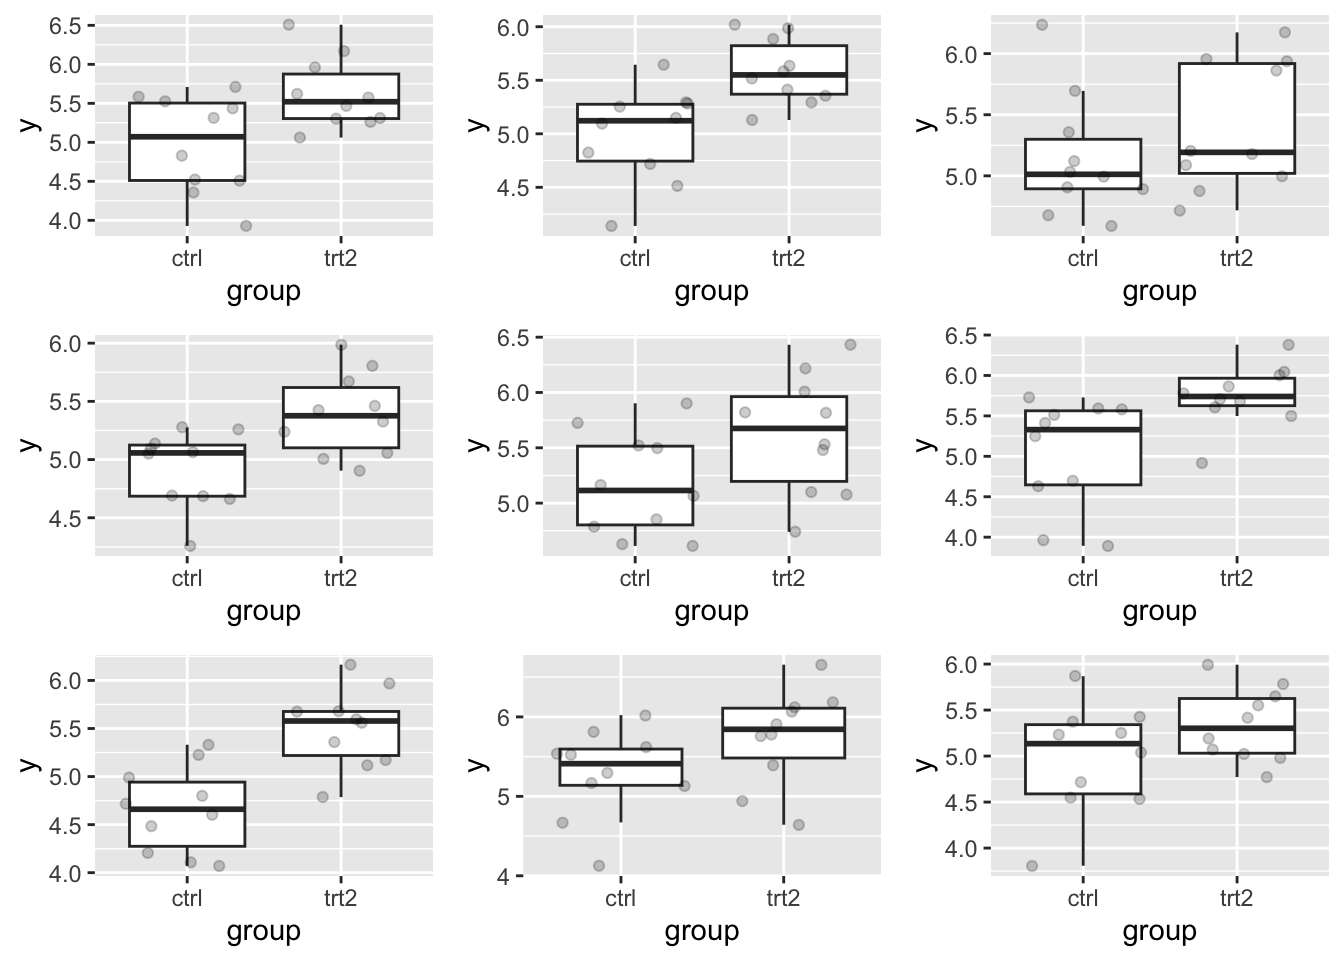
\includegraphics{introduction_files/figure-latex/unnamed-chunk-8-1.pdf}

\begin{Shaded}
\begin{Highlighting}[]
\NormalTok{p2}
\end{Highlighting}
\end{Shaded}

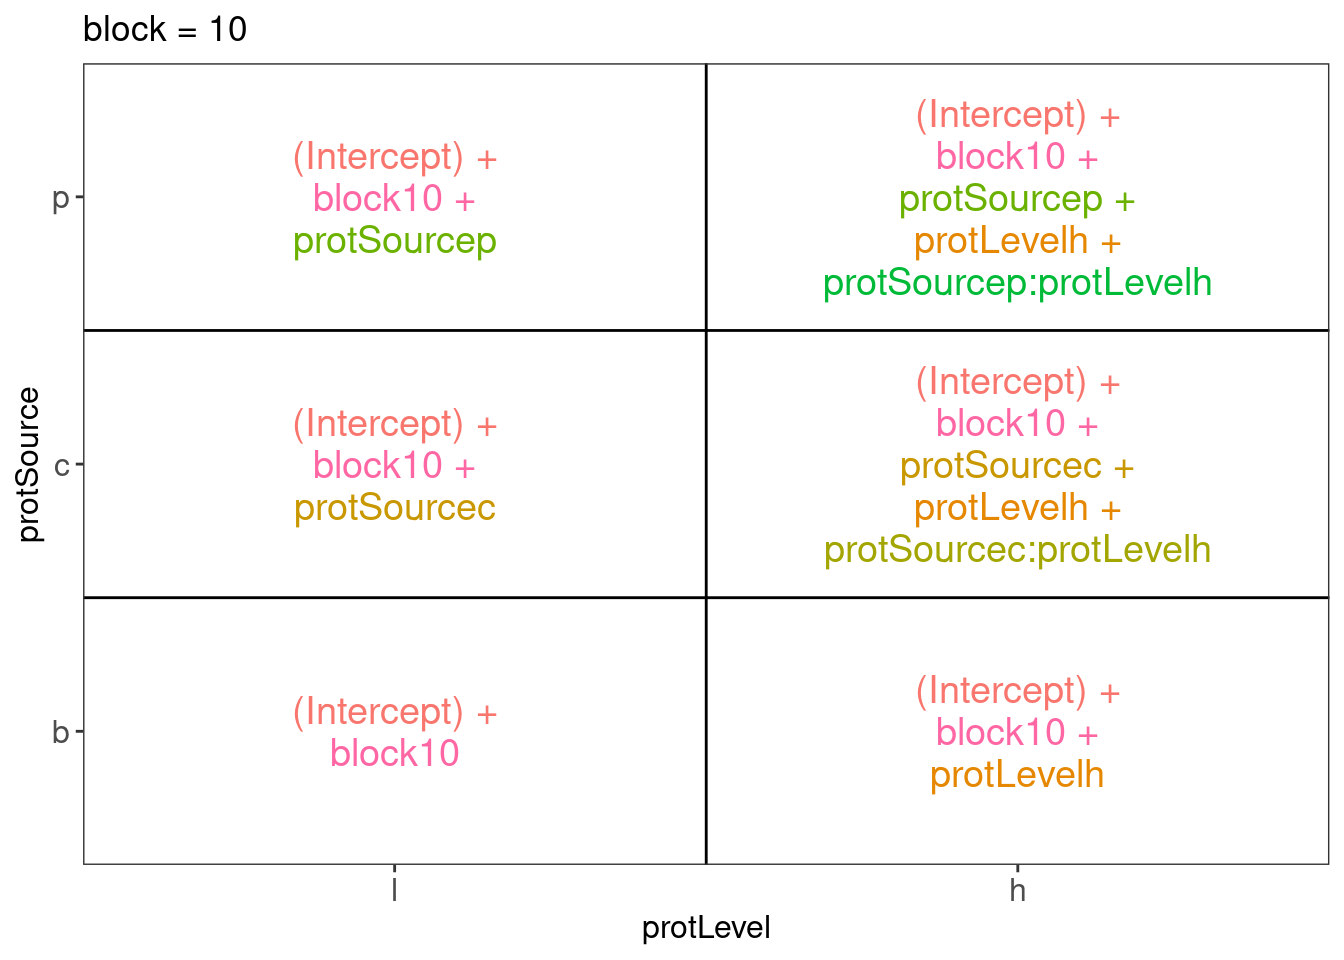
\includegraphics{introduction_files/figure-latex/unnamed-chunk-8-2.pdf}

\hypertarget{onderzoeksvraag}{%
\subsection{Onderzoeksvraag}\label{onderzoeksvraag}}

De onderzoekers wensen het effect te kennen van roken op de long
capaciteit van jongeren.

\hypertarget{hoe-modelleren-we-de-data}{%
\subsection{Hoe modelleren we de
data?}\label{hoe-modelleren-we-de-data}}

\begin{itemize}
\tightlist
\item
  \(x_i\): dummy variabele voor rokerstatus voor subject \(i\):
  \(x_{i,1}=\begin{cases} 0& \text{niet-roker}\\ 1& \text{roker} \end{cases}\).
\end{itemize}

\[Y_i\vert x_i\sim N(\mu_i,\sigma^2)\]

via lineair model?

\[Y_i = \beta_0 + \beta_1 x_i + \epsilon_i \text{ met } \epsilon_i\sim N(0,\sigma^2)\]

Vertaal de onderzoeksvraag naar de model parameters?

\begin{Shaded}
\begin{Highlighting}[]
\FunctionTok{library}\NormalTok{(ExploreModelMatrix)}

\NormalTok{lm1 }\OtherTok{\textless{}{-}} \FunctionTok{lm}\NormalTok{(fev}\SpecialCharTok{\textasciitilde{}}\NormalTok{smoking, fev)}
\NormalTok{lm1 }
\end{Highlighting}
\end{Shaded}

\begin{verbatim}
## 
## Call:
## lm(formula = fev ~ smoking, data = fev)
## 
## Coefficients:
## (Intercept)     smoking1  
##      2.6346       0.6054
\end{verbatim}

\begin{Shaded}
\begin{Highlighting}[]
\NormalTok{explMx }\OtherTok{\textless{}{-}} \FunctionTok{VisualizeDesign}\NormalTok{(fev,}\AttributeTok{designFormula =} \SpecialCharTok{\textasciitilde{}}\NormalTok{smoking)}
\NormalTok{explMx}\SpecialCharTok{$}\NormalTok{plotlist}
\end{Highlighting}
\end{Shaded}

\begin{verbatim}
## [[1]]
\end{verbatim}

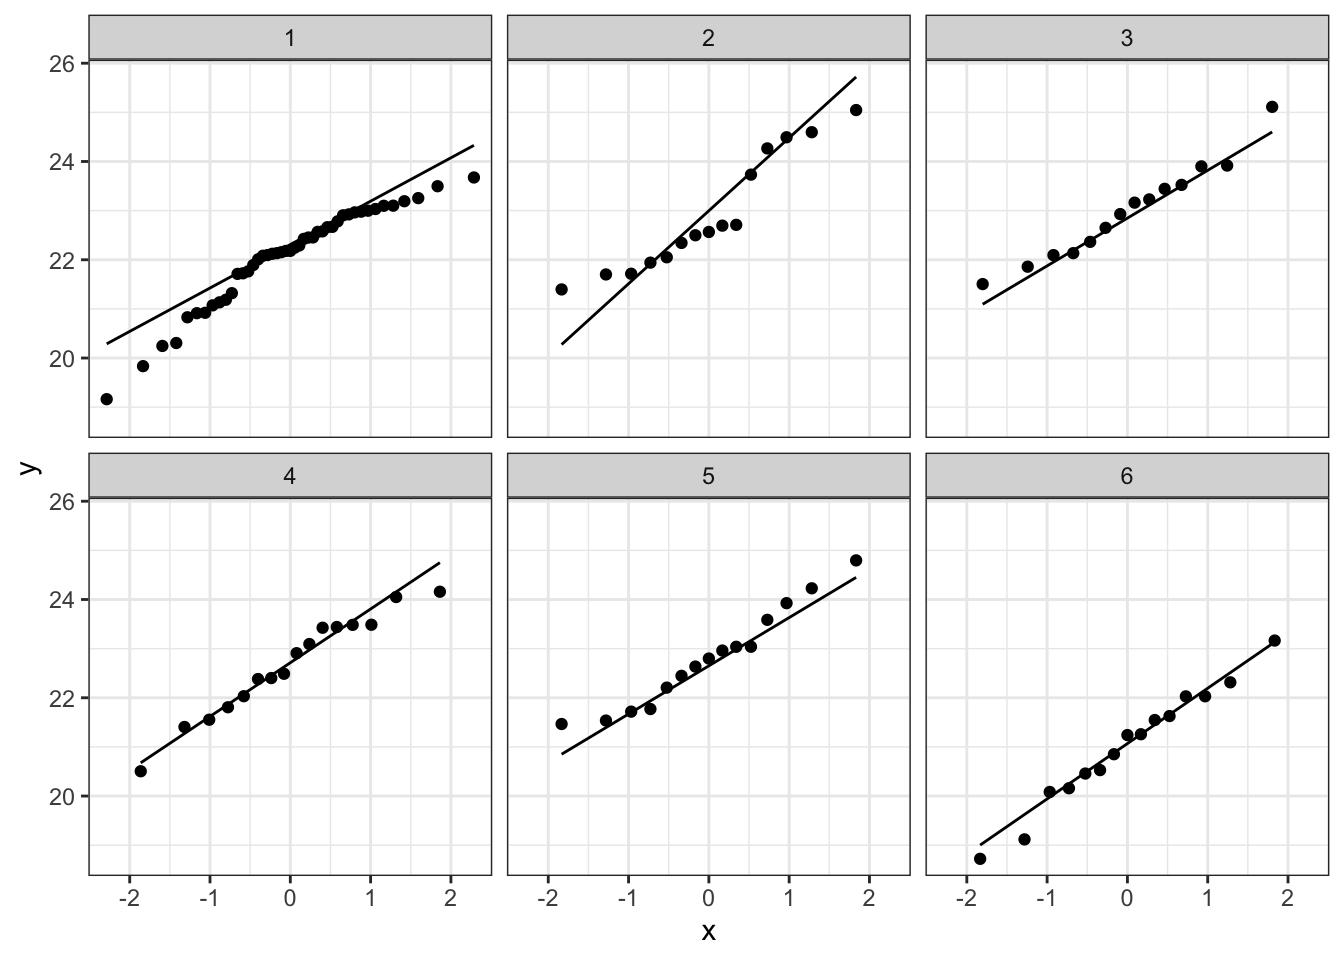
\includegraphics{introduction_files/figure-latex/unnamed-chunk-9-1.pdf}

\begin{itemize}
\item
  Vertaal de onderzoeksvraag naar een parameter in het model.
\item
  Effectgrootte:
\end{itemize}

\[\mu_1-\mu_0 = \beta_0+\beta_1 - \beta_0 = \beta_1\]

\hypertarget{schatten-van-de-effectgrootte-en-de-standard-error}{%
\subsubsection{Schatten van de effectgrootte en de standard
error}\label{schatten-van-de-effectgrootte-en-de-standard-error}}

\begin{Shaded}
\begin{Highlighting}[]
\FunctionTok{summary}\NormalTok{(lm1)}
\end{Highlighting}
\end{Shaded}

\begin{verbatim}
## 
## Call:
## lm(formula = fev ~ smoking, data = fev)
## 
## Residuals:
##     Min      1Q  Median      3Q     Max 
## -1.5460 -0.5754 -0.1036  0.4474  3.1584 
## 
## Coefficients:
##             Estimate Std. Error t value Pr(>|t|)    
## (Intercept)  2.63463    0.03469  75.943  < 2e-16 ***
## smoking1     0.60541    0.10935   5.537  4.6e-08 ***
## ---
## Signif. codes:  0 '***' 0.001 '**' 0.01 '*' 0.05 '.' 0.1 ' ' 1
## 
## Residual standard error: 0.8099 on 604 degrees of freedom
## Multiple R-squared:  0.0483, Adjusted R-squared:  0.04672 
## F-statistic: 30.65 on 1 and 604 DF,  p-value: 4.603e-08
\end{verbatim}

\hypertarget{statistische-inferentie}{%
\subsection{Statistische Inferentie?}\label{statistische-inferentie}}

\hypertarget{nul-en-alternatieve-hypothese}{%
\subsubsection{Nul en alternatieve
hypothese?}\label{nul-en-alternatieve-hypothese}}

We wensen de \textbf{alternatieve hypothese} \(H_1\) aan te tonen: er is
een effect van roken op de longcapaciteit van jongeren. We vertalen dit
naar ons model:

\begin{itemize}
\tightlist
\item
  \(H_1\): Gemiddeld is de longcapaciteit van niet-rokende en rokende
  jongeren verschillend \[\beta \neq 0\]
\end{itemize}

We kunnen op basis van data echter een hypothese niet bewijzen. Daarom
zullen we het omgekeerde falsifiëren:

\begin{itemize}
\item
  \(H_0\): Gemiddeld is de longcapaciteit van niet-rokende en rokende
  jongeren gelijk \[\beta = 0\]
\item
  Hoe falsifieren we \(H_0\)?
\end{itemize}

\begin{center}\rule{0.5\linewidth}{0.5pt}\end{center}

\begin{Shaded}
\begin{Highlighting}[]
\FunctionTok{summary}\NormalTok{(lm1)}
\end{Highlighting}
\end{Shaded}

\begin{verbatim}
## 
## Call:
## lm(formula = fev ~ smoking, data = fev)
## 
## Residuals:
##     Min      1Q  Median      3Q     Max 
## -1.5460 -0.5754 -0.1036  0.4474  3.1584 
## 
## Coefficients:
##             Estimate Std. Error t value Pr(>|t|)    
## (Intercept)  2.63463    0.03469  75.943  < 2e-16 ***
## smoking1     0.60541    0.10935   5.537  4.6e-08 ***
## ---
## Signif. codes:  0 '***' 0.001 '**' 0.01 '*' 0.05 '.' 0.1 ' ' 1
## 
## Residual standard error: 0.8099 on 604 degrees of freedom
## Multiple R-squared:  0.0483, Adjusted R-squared:  0.04672 
## F-statistic: 30.65 on 1 and 604 DF,  p-value: 4.603e-08
\end{verbatim}

\begin{itemize}
\item
  Hoe waarschijnlijk is het om een effectgrootte (test-statistiek) te
  vinden die meer extreem is dan wat we observeerden in een random
  steekproef wanneer de nulhypothese waar is.
\item
  Als we aannames kunnen doen over de verdelingen van de gegevens,
  kennen we de verdeling van de test statistiek en kunnen we die kans
  berekenen: \textbf{p-waarde}.
\item
  Als de p-waarde lager is dan het nominale significantie-niveau
  \(\alpha\) verwerpen we de null hypothese.
\end{itemize}

\emph{We controleren de kans op het maken van een vals positieve
conclusie op het \(\alpha\)-niveau (type I fout)}

\begin{itemize}
\tightlist
\item
  De p-value is enkel correct als de onderliggende aannames geldig zijn.
\end{itemize}

\begin{Shaded}
\begin{Highlighting}[]
\NormalTok{p1}
\end{Highlighting}
\end{Shaded}

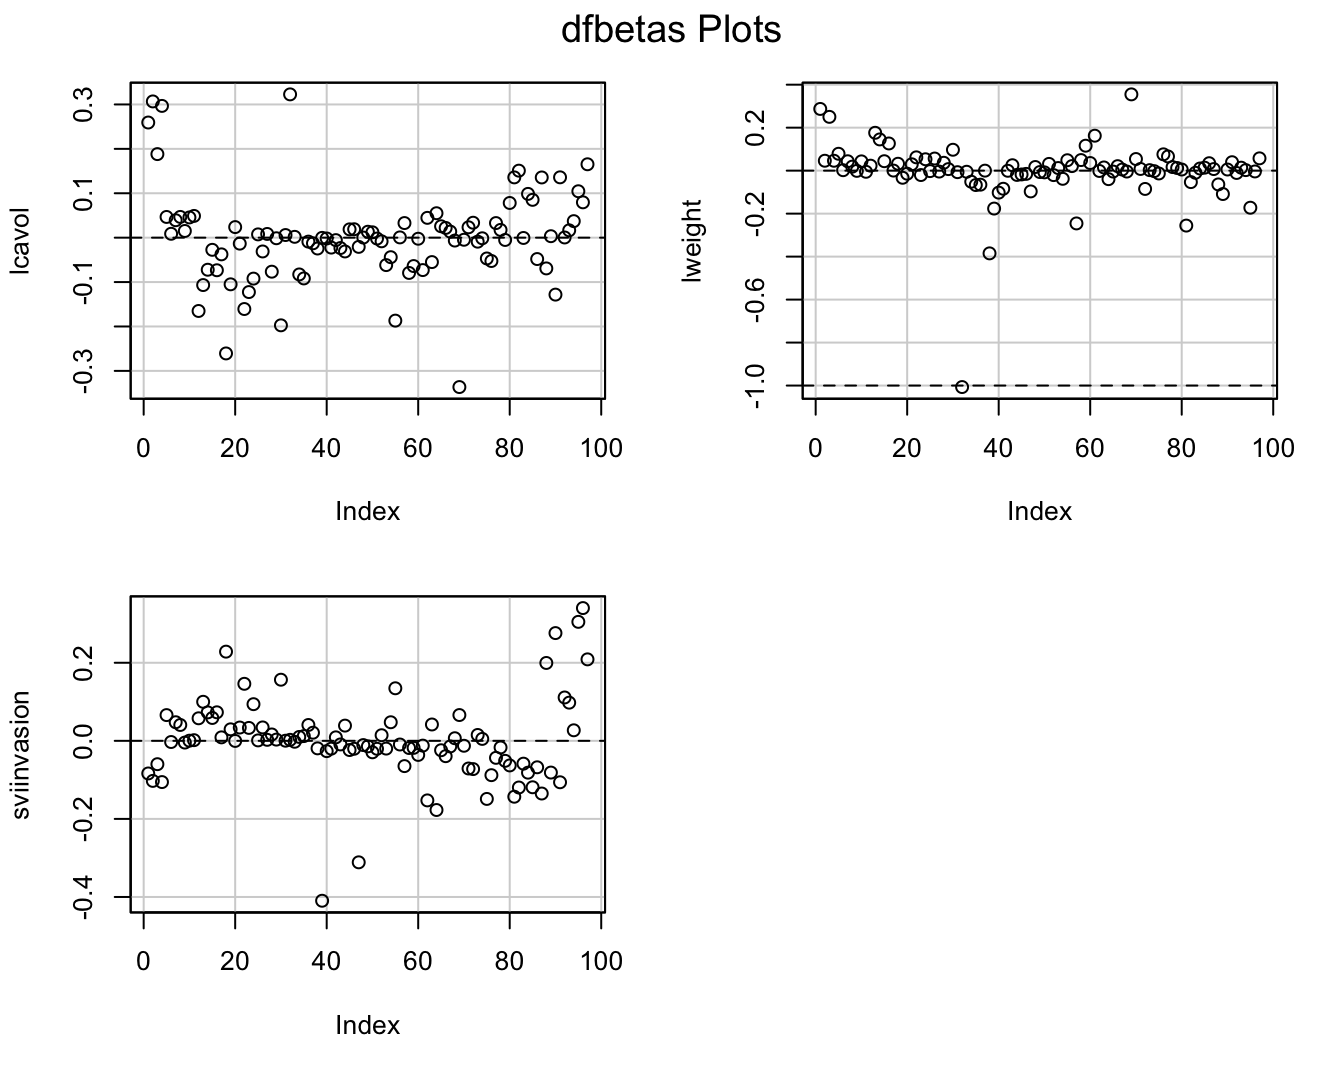
\includegraphics{introduction_files/figure-latex/unnamed-chunk-12-1.pdf}

\begin{Shaded}
\begin{Highlighting}[]
\NormalTok{p2}
\end{Highlighting}
\end{Shaded}

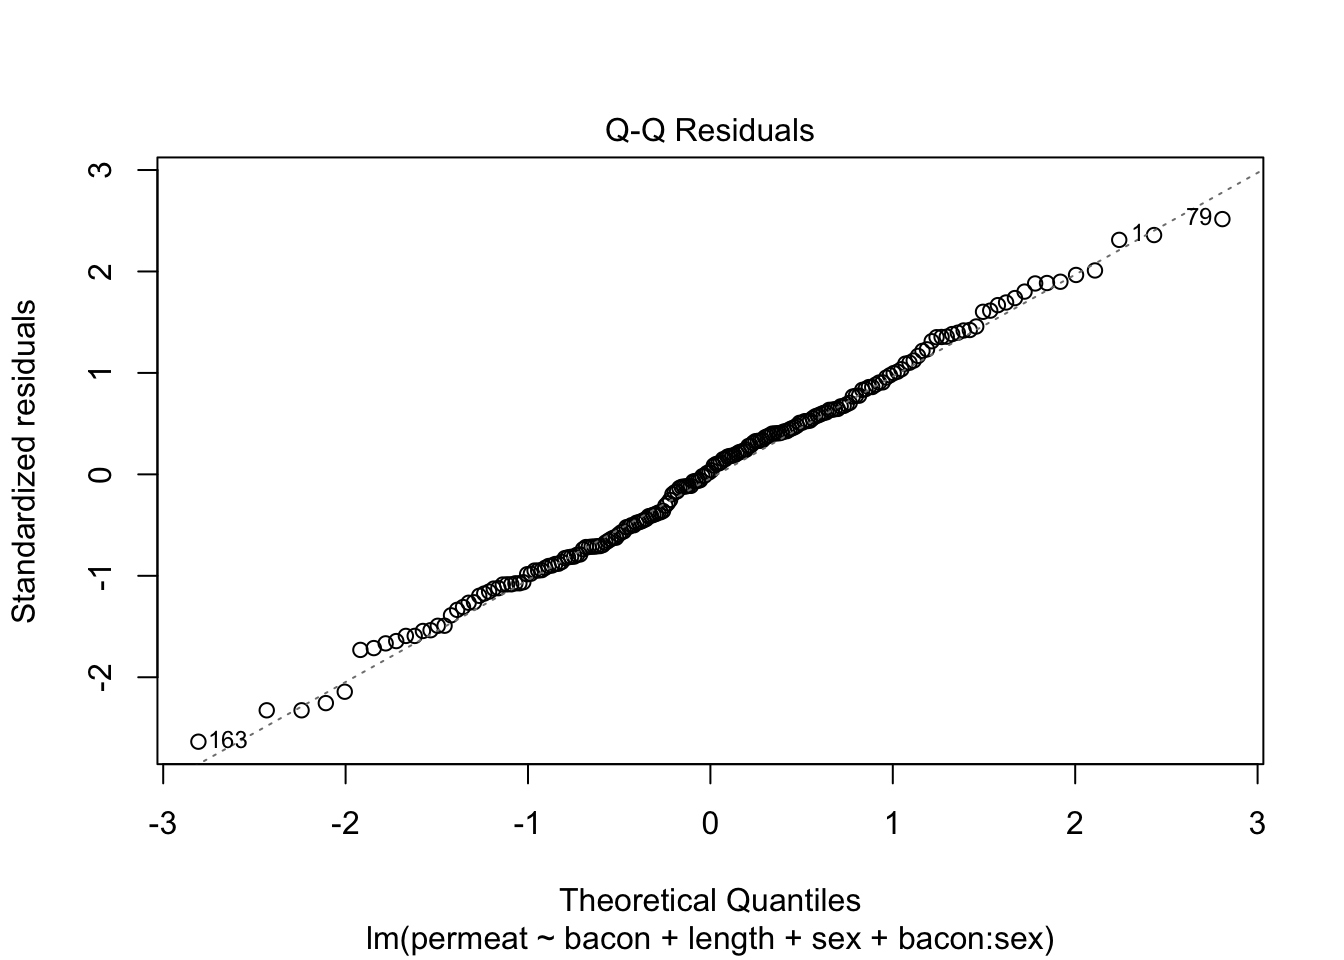
\includegraphics{introduction_files/figure-latex/unnamed-chunk-12-2.pdf}

\begin{itemize}
\tightlist
\item
  Biologische metingen zijn dikwijls niet normaal verdeeld.
\item
  Dikwijls zijn de gegevens na log-transformatie meer normaal
  verdeeld.\\
\item
  Verschillen op log schaal:
\end{itemize}

\[
\log_2(S) - \log_2(NS) = \log_2 \frac{S}{NS} = \log_2 FC_{\frac{S}{NS}}
\]

\begin{center}\rule{0.5\linewidth}{0.5pt}\end{center}

\hypertarget{log-transformation}{%
\subsection{Log transformation}\label{log-transformation}}

\begin{Shaded}
\begin{Highlighting}[]
\NormalTok{p1 }\OtherTok{\textless{}{-}}\NormalTok{ fev }\SpecialCharTok{\%\textgreater{}\%}
  \FunctionTok{ggplot}\NormalTok{(}\FunctionTok{aes}\NormalTok{(}\AttributeTok{x=}\NormalTok{smoking,}\AttributeTok{y=}\FunctionTok{log2}\NormalTok{(fev))) }\SpecialCharTok{+}
  \FunctionTok{geom\_boxplot}\NormalTok{(}\AttributeTok{outlier.shape=}\ConstantTok{NA}\NormalTok{) }\SpecialCharTok{+}
  \FunctionTok{geom\_jitter}\NormalTok{(}\AttributeTok{alpha=}\NormalTok{.}\DecValTok{2}\NormalTok{)}

\NormalTok{p2 }\OtherTok{\textless{}{-}}\NormalTok{ fev }\SpecialCharTok{\%\textgreater{}\%}
  \FunctionTok{ggplot}\NormalTok{(}\FunctionTok{aes}\NormalTok{(}\AttributeTok{sample=}\FunctionTok{log2}\NormalTok{(fev))) }\SpecialCharTok{+}
  \FunctionTok{geom\_qq}\NormalTok{() }\SpecialCharTok{+}
  \FunctionTok{geom\_qq\_line}\NormalTok{() }\SpecialCharTok{+}
  \FunctionTok{facet\_wrap}\NormalTok{(}\SpecialCharTok{\textasciitilde{}}\NormalTok{smoking)}
\NormalTok{p1}
\end{Highlighting}
\end{Shaded}

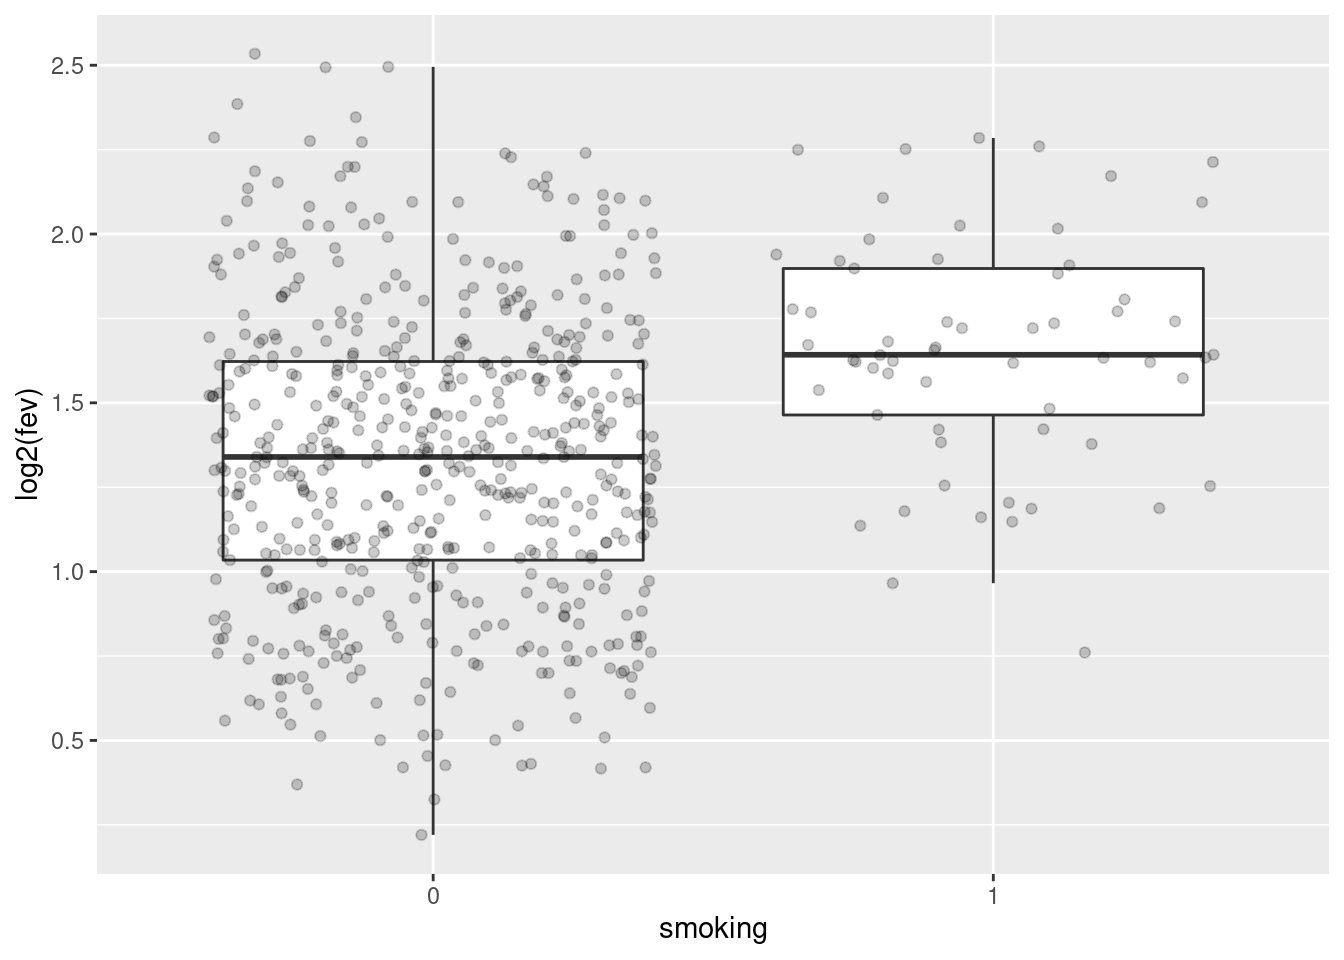
\includegraphics{introduction_files/figure-latex/unnamed-chunk-13-1.pdf}

\begin{Shaded}
\begin{Highlighting}[]
\NormalTok{p2}
\end{Highlighting}
\end{Shaded}

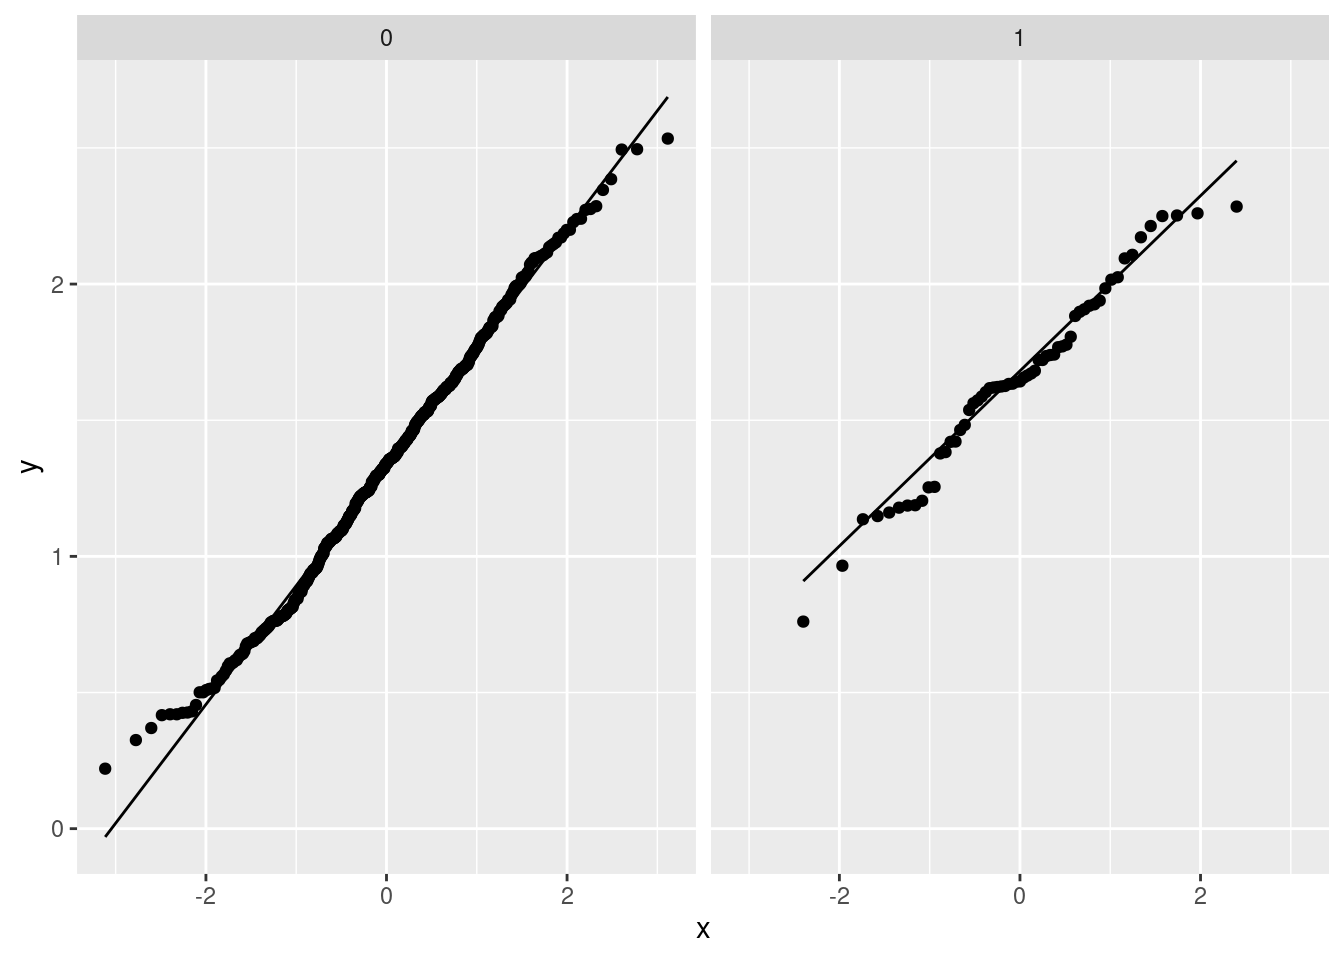
\includegraphics{introduction_files/figure-latex/unnamed-chunk-13-2.pdf}

\begin{Shaded}
\begin{Highlighting}[]
\NormalTok{lm1 }\OtherTok{\textless{}{-}} \FunctionTok{lm}\NormalTok{(}\FunctionTok{log2}\NormalTok{(fev)}\SpecialCharTok{\textasciitilde{}}\NormalTok{smoking,fev)}
\FunctionTok{summary}\NormalTok{(lm1)}
\end{Highlighting}
\end{Shaded}

\begin{verbatim}
## 
## Call:
## lm(formula = log2(fev) ~ smoking, data = fev)
## 
## Residuals:
##      Min       1Q   Median       3Q      Max 
## -1.11108 -0.28248  0.00693  0.28172  1.20290 
## 
## Coefficients:
##             Estimate Std. Error t value Pr(>|t|)    
## (Intercept)  1.33141    0.01833  72.649  < 2e-16 ***
## smoking1     0.32592    0.05776   5.642 2.58e-08 ***
## ---
## Signif. codes:  0 '***' 0.001 '**' 0.01 '*' 0.05 '.' 0.1 ' ' 1
## 
## Residual standard error: 0.4278 on 604 degrees of freedom
## Multiple R-squared:  0.05007,    Adjusted R-squared:  0.0485 
## F-statistic: 31.84 on 1 and 604 DF,  p-value: 2.582e-08
\end{verbatim}

\begin{Shaded}
\begin{Highlighting}[]
\DecValTok{2}\SpecialCharTok{\^{}}\NormalTok{(lm1}\SpecialCharTok{$}\NormalTok{coefficients)}
\end{Highlighting}
\end{Shaded}

\begin{verbatim}
## (Intercept)    smoking1 
##    2.516487    1.253463
\end{verbatim}

\begin{Shaded}
\begin{Highlighting}[]
\DecValTok{2}\SpecialCharTok{\^{}}\NormalTok{(}\FunctionTok{confint}\NormalTok{(lm1))}
\end{Highlighting}
\end{Shaded}

\begin{verbatim}
##                2.5 %   97.5 %
## (Intercept) 2.454484 2.580058
## smoking1    1.158676 1.356004
\end{verbatim}

\begin{Shaded}
\begin{Highlighting}[]
\DocumentationTok{\#\# verschil in variantie {-}{-}\textgreater{} Welch t{-}test}

\NormalTok{fevttest }\OtherTok{\textless{}{-}} \FunctionTok{t.test}\NormalTok{(}\FunctionTok{log2}\NormalTok{(fev)}\SpecialCharTok{\textasciitilde{}}\NormalTok{smoking,fev)}
\DecValTok{2}\SpecialCharTok{\^{}}\NormalTok{(fevttest}\SpecialCharTok{$}\NormalTok{estimate[}\DecValTok{2}\NormalTok{]}\SpecialCharTok{{-}}\NormalTok{fevttest}\SpecialCharTok{$}\NormalTok{estimate[}\DecValTok{1}\NormalTok{])}
\end{Highlighting}
\end{Shaded}

\begin{verbatim}
## mean in group 1 
##        1.253463
\end{verbatim}

\begin{Shaded}
\begin{Highlighting}[]
\DecValTok{2}\SpecialCharTok{\^{}{-}}\NormalTok{fevttest}\SpecialCharTok{$}\NormalTok{conf.int }\SpecialCharTok{\%\textgreater{}\%}\NormalTok{ sort}
\end{Highlighting}
\end{Shaded}

\begin{verbatim}
## [1] 1.174285 1.337979
\end{verbatim}

\hypertarget{conclusie}{%
\subsection{Conclusie}\label{conclusie}}

\begin{itemize}
\item
  Er is een extreem significant verschil in gemiddelde longinhoud tussen
  rokende en niet-rokende jongeren (\(p << 0.001\)).
\item
  Gemiddelde is de longinhoud 1.25 keer groter bij rokerende dan bij
  niet-rokende jongeren (95\% BI {[}1.17, 1.34{]} .
\end{itemize}

\begin{center}\rule{0.5\linewidth}{0.5pt}\end{center}

\begin{itemize}
\tightlist
\item
  Probleem!
\item
  Observationele studie
\item
  Confounding!
\end{itemize}

\begin{center}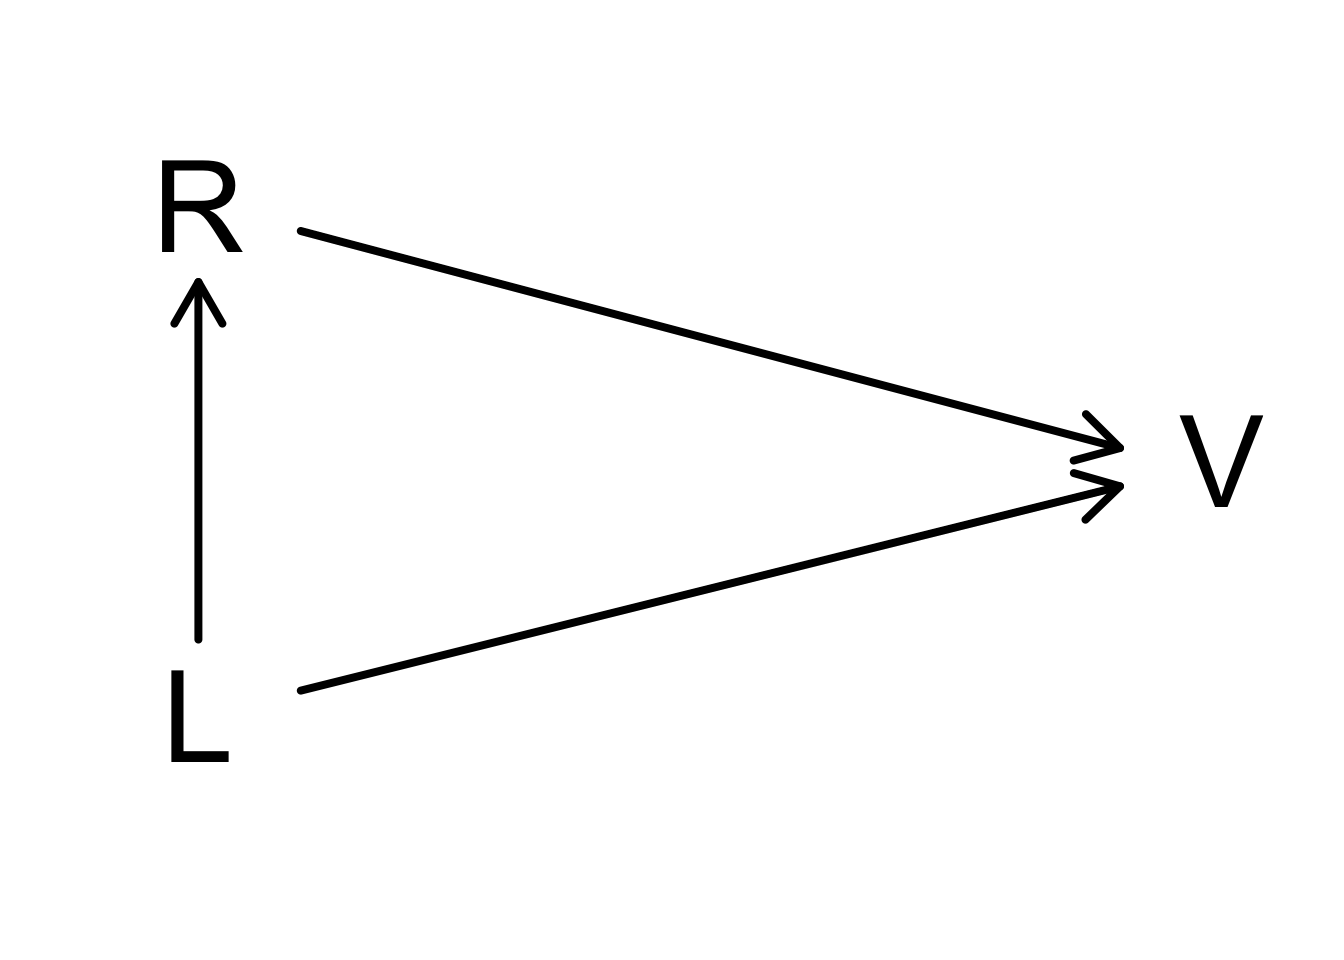
\includegraphics[width=0.5\linewidth]{introduction_files/figure-latex/unnamed-chunk-14-1} \end{center}

\begin{itemize}
\tightlist
\item
  Leeftijd (L) is heeft een invloed op het rookgedrag (R) en op de
  longinhoud (V)!
\item
  Als we leeftijd niet meenemen in de analyse dan kan het zijn dat de
  associatie tussen rookgedrag en de longinhoud vertekend is omdat
  rokers en niet-rokers niet alleen in rookgedrag maar ook in leeftijd
  verschillen!
\item
  Confounding is een probleem die typisch optreedt in observationele
  studies!
\end{itemize}

\begin{Shaded}
\begin{Highlighting}[]
\FunctionTok{library}\NormalTok{(GGally)}

\NormalTok{fev }\SpecialCharTok{\%\textgreater{}\%} 
  \FunctionTok{mutate}\NormalTok{(}\AttributeTok{lfev=}\FunctionTok{log2}\NormalTok{(fev)) }\SpecialCharTok{\%\textgreater{}\%} 
\NormalTok{  dplyr}\SpecialCharTok{::}\FunctionTok{select}\NormalTok{(smoking,gender,age,height\_cm,lfev) }\SpecialCharTok{\%\textgreater{}\%} 
  \FunctionTok{ggpairs}\NormalTok{()}
\end{Highlighting}
\end{Shaded}

\begin{verbatim}
## `stat_bin()` using `bins = 30`. Pick better value with `binwidth`.
## `stat_bin()` using `bins = 30`. Pick better value with `binwidth`.
## `stat_bin()` using `bins = 30`. Pick better value with `binwidth`.
## `stat_bin()` using `bins = 30`. Pick better value with `binwidth`.
## `stat_bin()` using `bins = 30`. Pick better value with `binwidth`.
## `stat_bin()` using `bins = 30`. Pick better value with `binwidth`.
\end{verbatim}

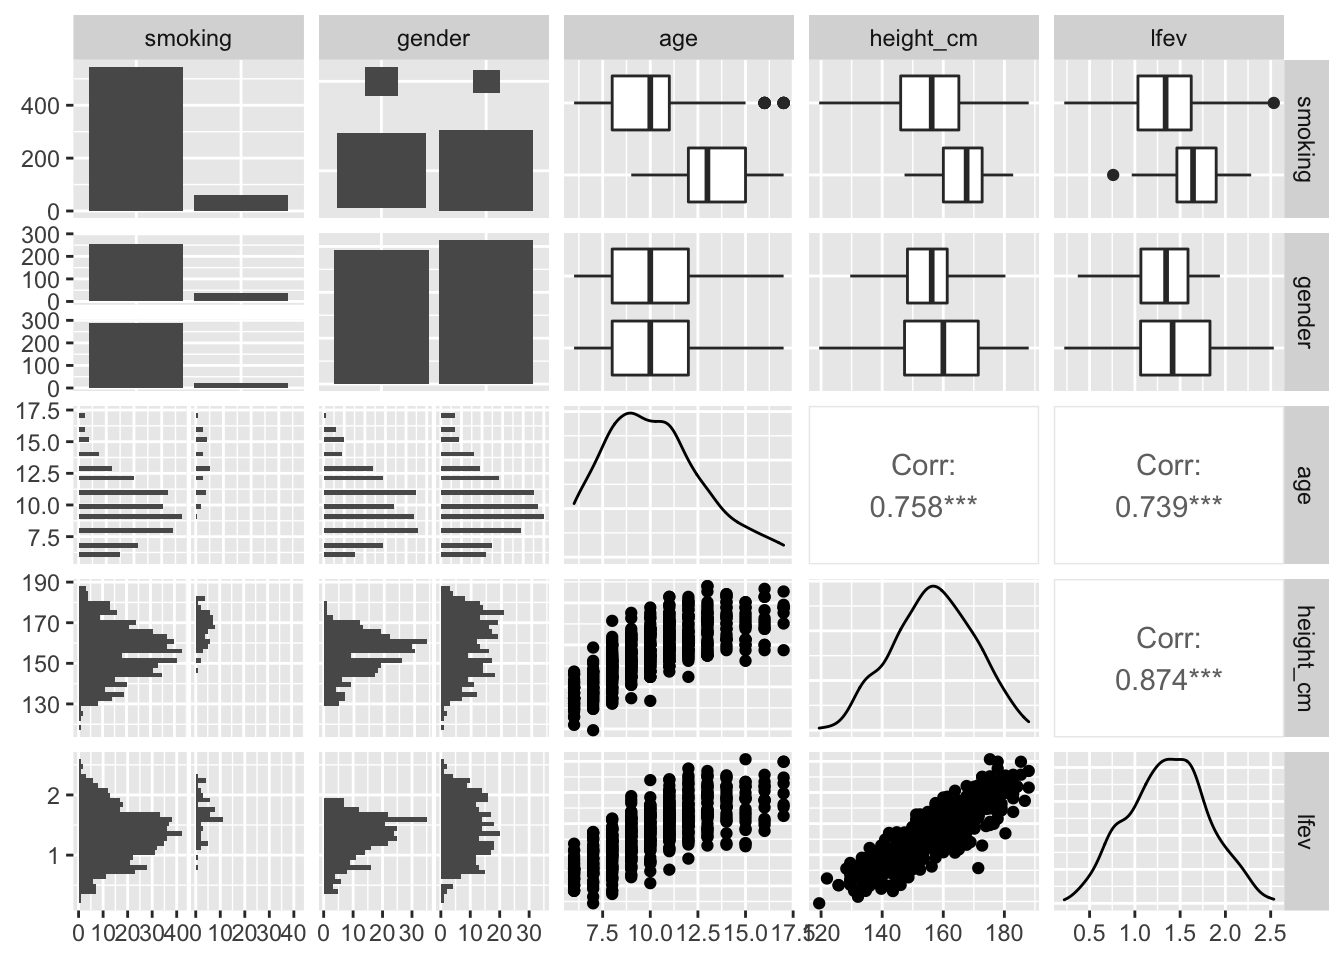
\includegraphics{introduction_files/figure-latex/unnamed-chunk-15-1.pdf}

Een betere data exploratie:

\begin{Shaded}
\begin{Highlighting}[]
\NormalTok{fev }\SpecialCharTok{\%\textgreater{}\%}
  \FunctionTok{ggplot}\NormalTok{(}\FunctionTok{aes}\NormalTok{(}\AttributeTok{x=}\FunctionTok{as.factor}\NormalTok{(age),}\AttributeTok{y=}\NormalTok{fev,}\AttributeTok{fill=}\NormalTok{smoking)) }\SpecialCharTok{+}
  \FunctionTok{geom\_boxplot}\NormalTok{(}\AttributeTok{outlier.shape=}\ConstantTok{NA}\NormalTok{) }\SpecialCharTok{+}
  \FunctionTok{geom\_point}\NormalTok{(}\AttributeTok{size =} \FloatTok{0.1}\NormalTok{, }\AttributeTok{position =} \FunctionTok{position\_jitterdodge}\NormalTok{()) }\SpecialCharTok{+}
  \FunctionTok{theme\_bw}\NormalTok{() }\SpecialCharTok{+}
  \FunctionTok{scale\_fill\_manual}\NormalTok{(}\AttributeTok{values=}\FunctionTok{c}\NormalTok{(}\StringTok{"dimgrey"}\NormalTok{,}\StringTok{"firebrick"}\NormalTok{)) }\SpecialCharTok{+}
  \FunctionTok{ggtitle}\NormalTok{(}\StringTok{"Boxplot of FEV versus smoking, stratified on age and gender"}\NormalTok{) }\SpecialCharTok{+}
  \FunctionTok{ylab}\NormalTok{(}\StringTok{"fev (l)"}\NormalTok{) }\SpecialCharTok{+}
  \FunctionTok{xlab}\NormalTok{(}\StringTok{"age (years)"}\NormalTok{) }\SpecialCharTok{+} 
  \FunctionTok{facet\_grid}\NormalTok{(}\AttributeTok{rows =} \FunctionTok{vars}\NormalTok{(gender))}
\end{Highlighting}
\end{Shaded}

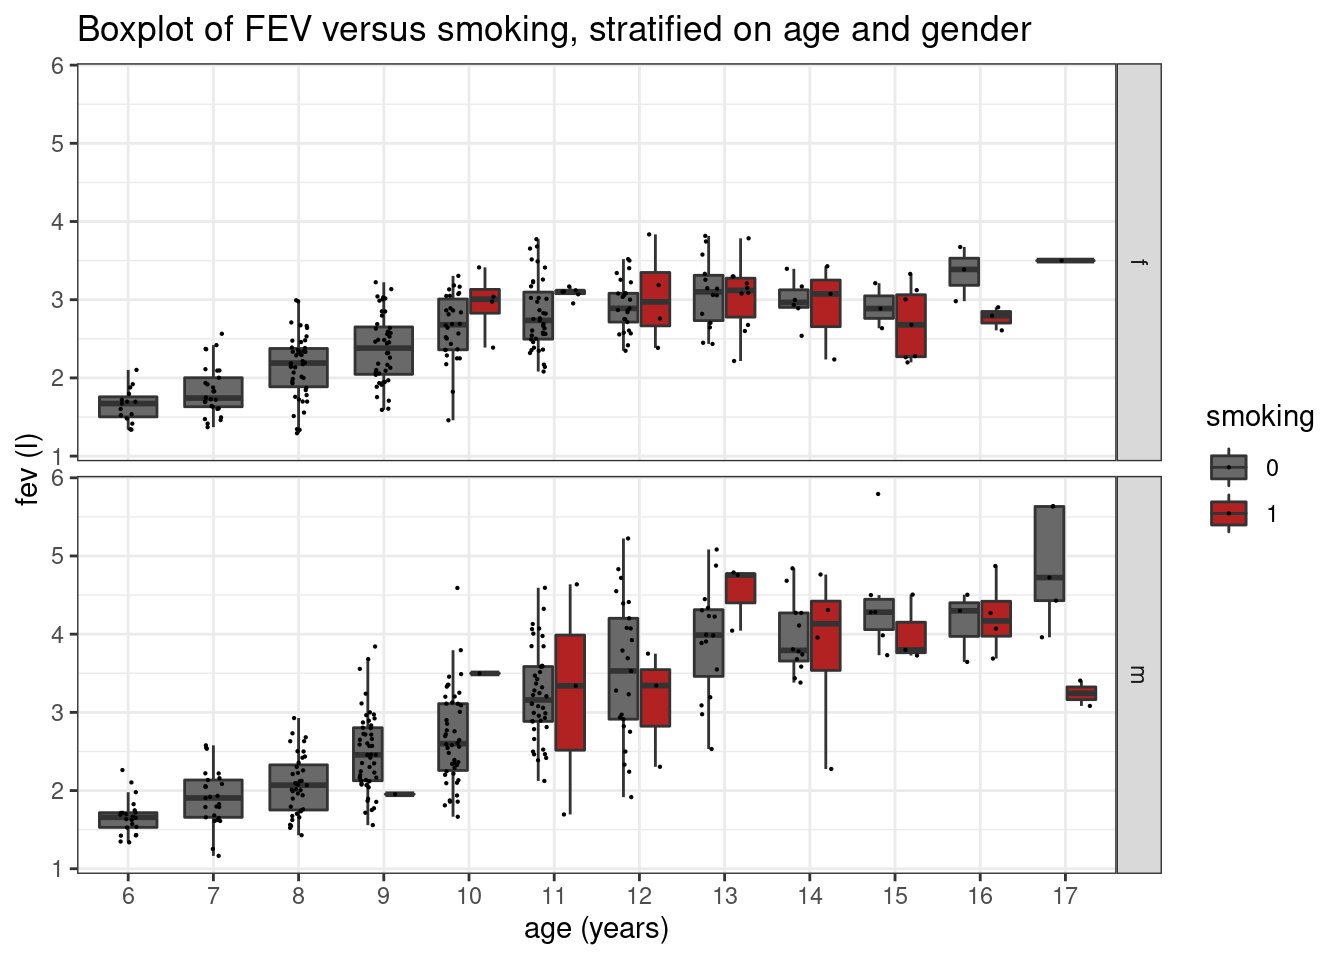
\includegraphics{introduction_files/figure-latex/unnamed-chunk-16-1.pdf}

\begin{center}\rule{0.5\linewidth}{0.5pt}\end{center}

\begin{itemize}
\tightlist
\item
  Hoe zouden we de associatie tussen leeftijd en fev kunnen modelleren?
\item
  We doen dit eerst enkel voor niet-rokende meisjes. Want er is ook een
  associatie tussen fev en geslacht.
\end{itemize}

\begin{Shaded}
\begin{Highlighting}[]
\NormalTok{lm2 }\OtherTok{\textless{}{-}}\NormalTok{ fev }\SpecialCharTok{\%\textgreater{}\%} 
  \FunctionTok{filter}\NormalTok{(gender}\SpecialCharTok{==}\StringTok{"f"} \SpecialCharTok{\&}\NormalTok{ smoking }\SpecialCharTok{==} \DecValTok{0}\NormalTok{) }\SpecialCharTok{\%\textgreater{}\%} 
  \FunctionTok{lm}\NormalTok{(}\FunctionTok{log2}\NormalTok{(fev)}\SpecialCharTok{\textasciitilde{}}\NormalTok{age,.)}

\FunctionTok{summary}\NormalTok{(lm2)}
\end{Highlighting}
\end{Shaded}

\begin{verbatim}
## 
## Call:
## lm(formula = log2(fev) ~ age, data = .)
## 
## Residuals:
##      Min       1Q   Median       3Q      Max 
## -0.75023 -0.16864  0.00122  0.18291  0.51611 
## 
## Coefficients:
##             Estimate Std. Error t value Pr(>|t|)    
## (Intercept) 0.150534   0.069503   2.166   0.0313 *  
## age         0.114369   0.007011  16.313   <2e-16 ***
## ---
## Signif. codes:  0 '***' 0.001 '**' 0.01 '*' 0.05 '.' 0.1 ' ' 1
## 
## Residual standard error: 0.252 on 253 degrees of freedom
## Multiple R-squared:  0.5126, Adjusted R-squared:  0.5107 
## F-statistic: 266.1 on 1 and 253 DF,  p-value: < 2.2e-16
\end{verbatim}

\begin{Shaded}
\begin{Highlighting}[]
\FunctionTok{plot}\NormalTok{(lm2)}
\end{Highlighting}
\end{Shaded}

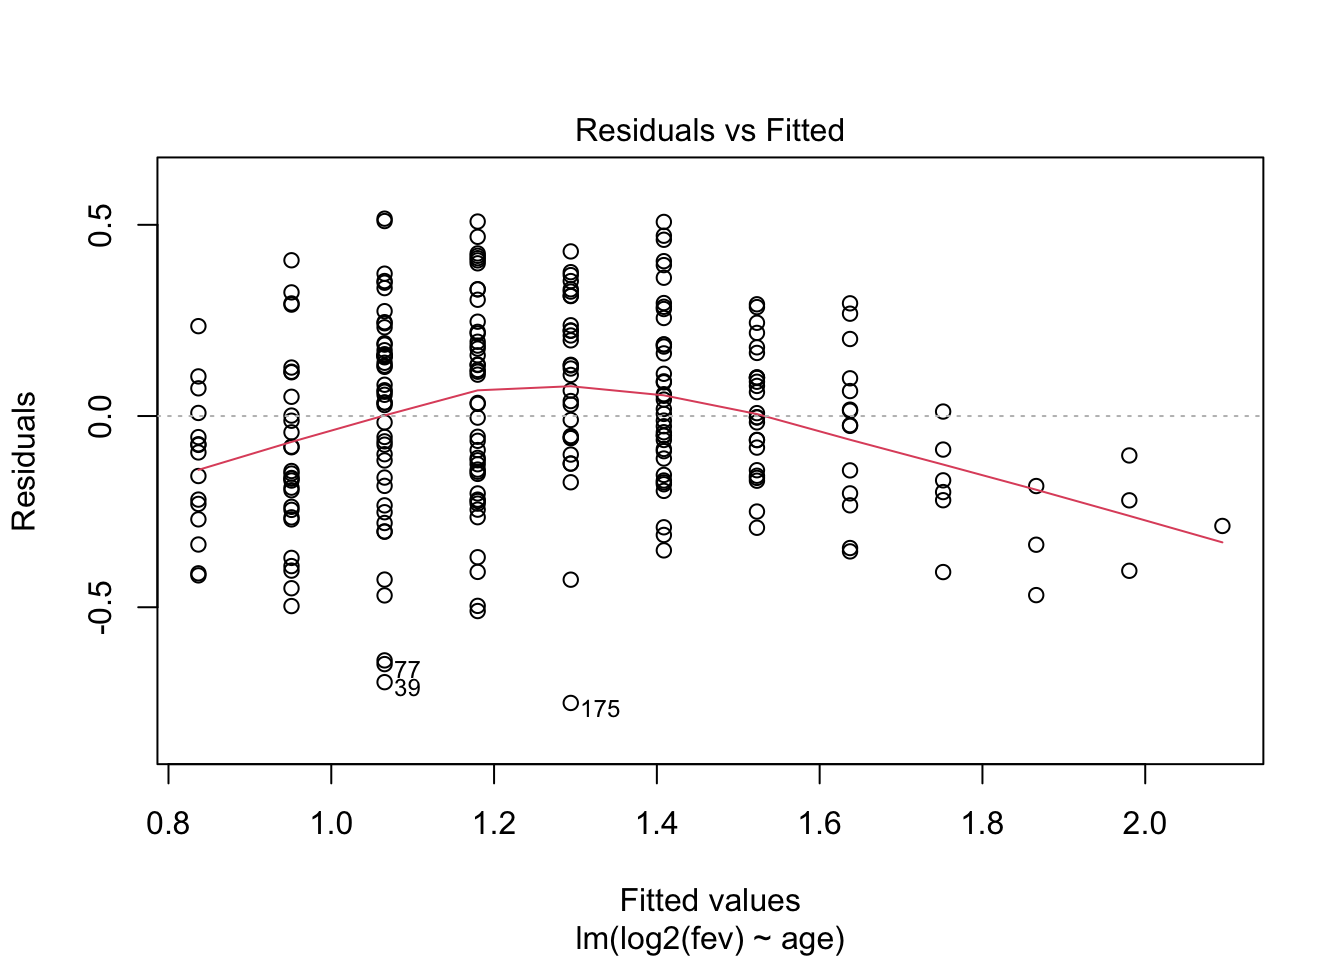
\includegraphics{introduction_files/figure-latex/unnamed-chunk-17-1.pdf}
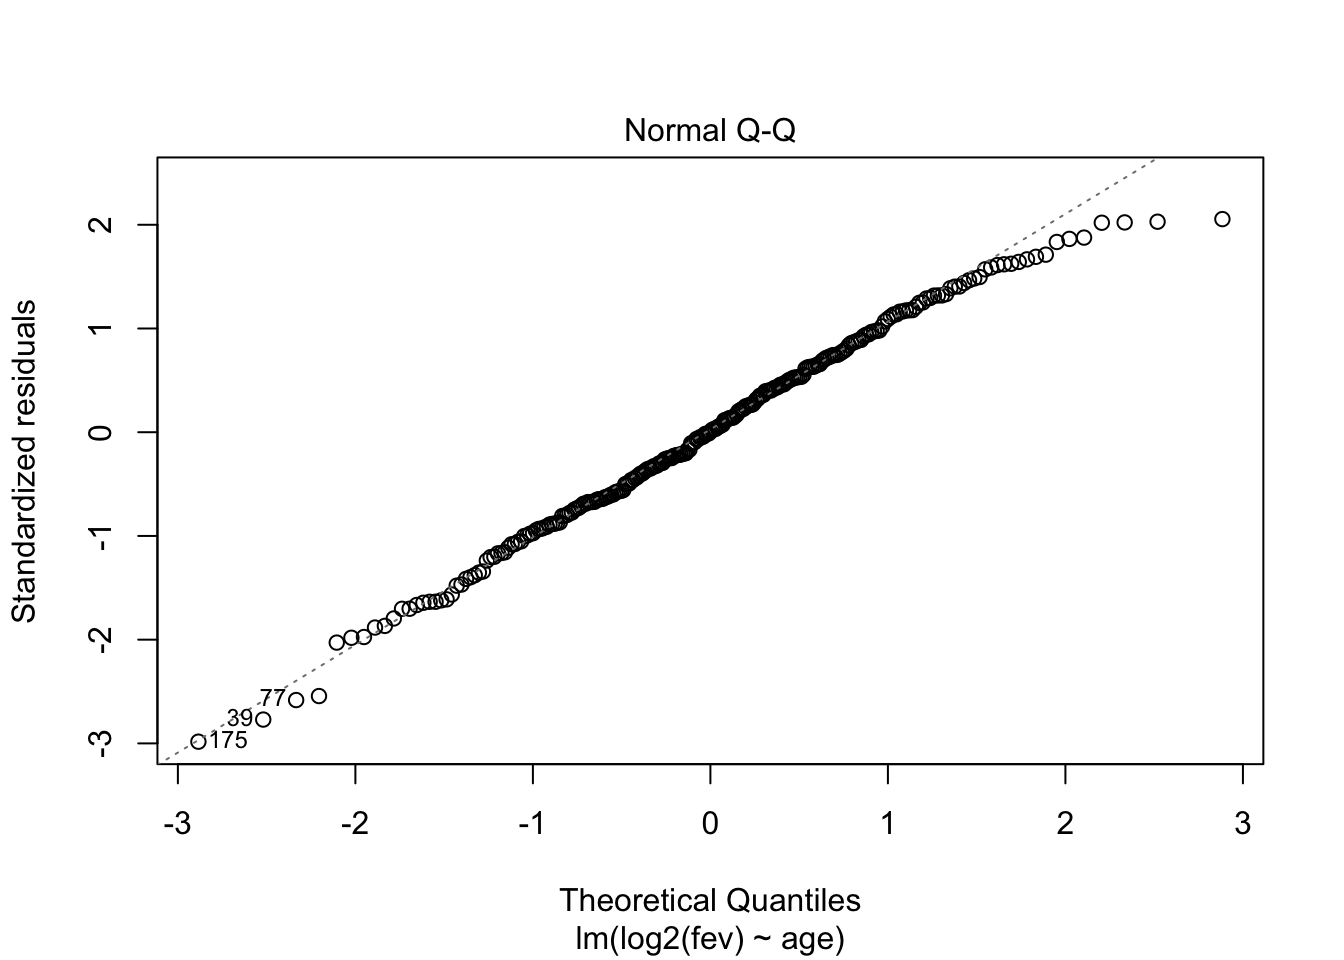
\includegraphics{introduction_files/figure-latex/unnamed-chunk-17-2.pdf}
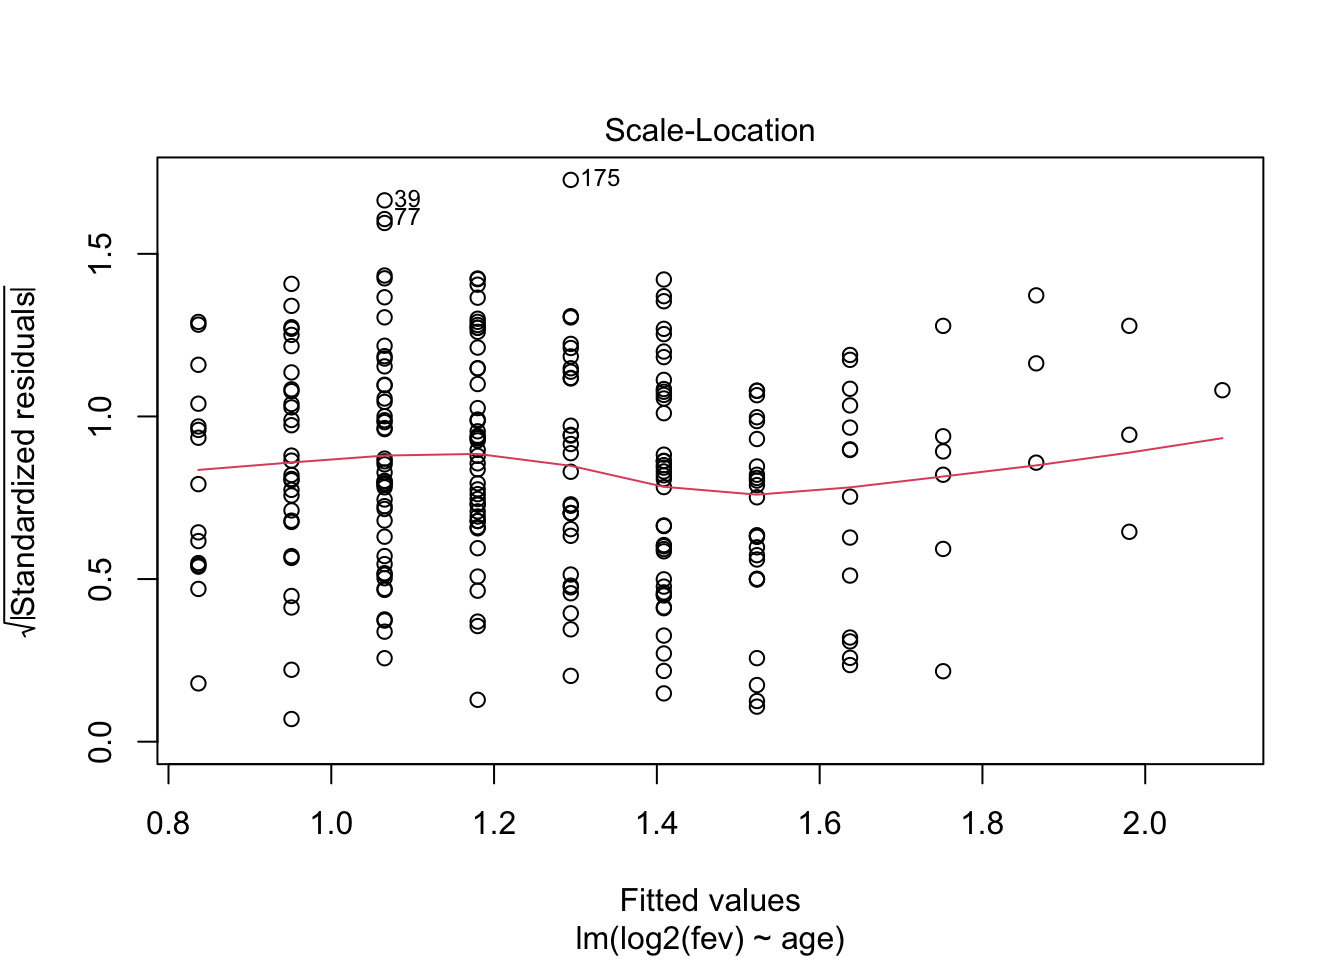
\includegraphics{introduction_files/figure-latex/unnamed-chunk-17-3.pdf}
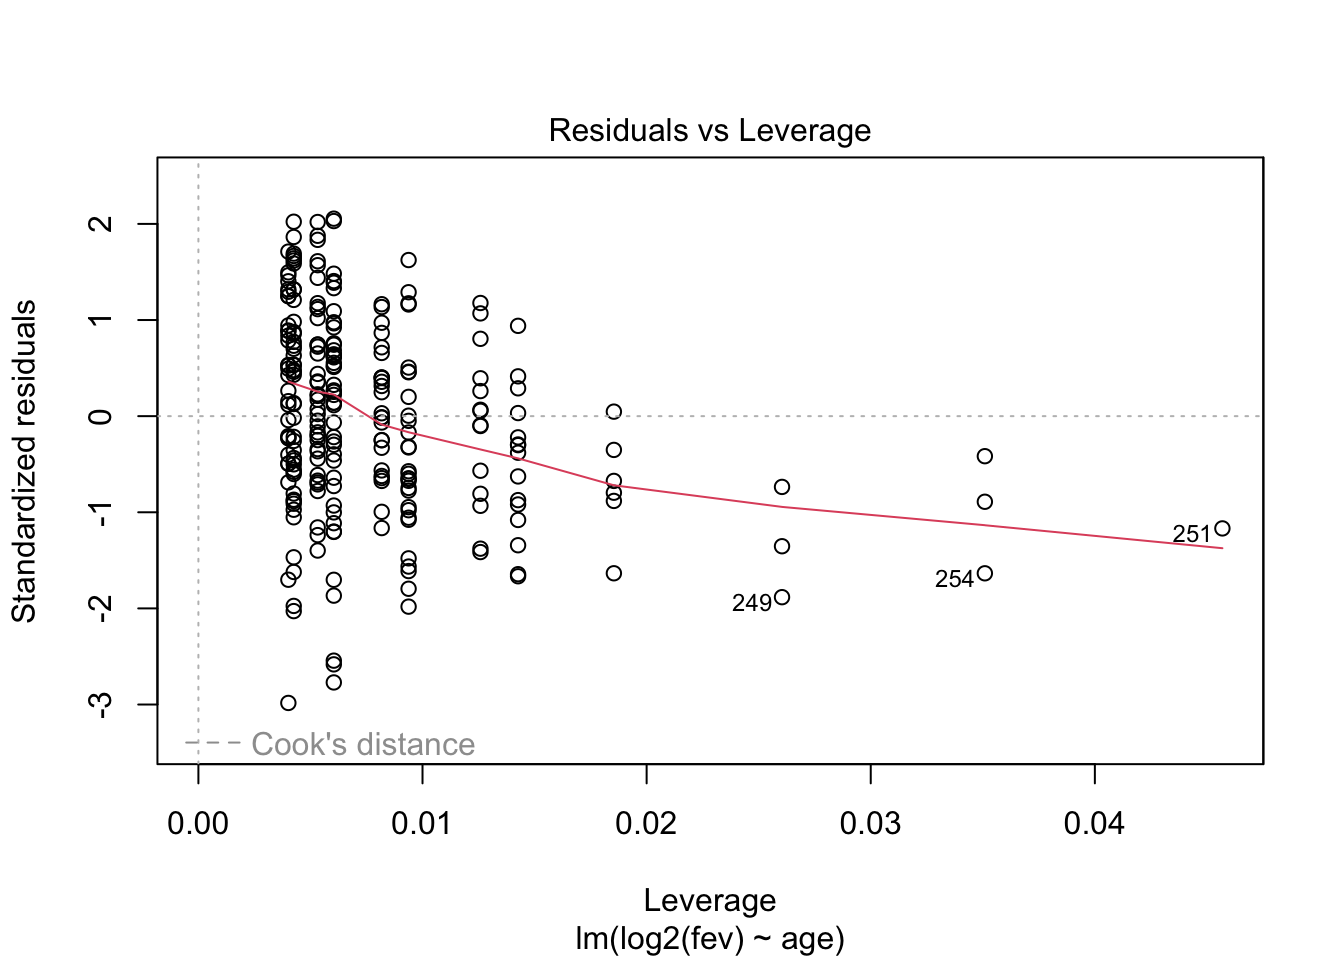
\includegraphics{introduction_files/figure-latex/unnamed-chunk-17-4.pdf}

\begin{Shaded}
\begin{Highlighting}[]
\NormalTok{fev }\SpecialCharTok{\%\textgreater{}\%} 
  \FunctionTok{filter}\NormalTok{(gender}\SpecialCharTok{==}\StringTok{"f"} \SpecialCharTok{\&}\NormalTok{ smoking }\SpecialCharTok{==} \DecValTok{0}\NormalTok{) }\SpecialCharTok{\%\textgreater{}\%} 
  \FunctionTok{ggplot}\NormalTok{(}\FunctionTok{aes}\NormalTok{(}\AttributeTok{x=}\NormalTok{age,}\AttributeTok{y=}\FunctionTok{log2}\NormalTok{(fev))) }\SpecialCharTok{+} 
  \FunctionTok{geom\_point}\NormalTok{() }\SpecialCharTok{+}
  \FunctionTok{geom\_smooth}\NormalTok{(}\AttributeTok{method =} \StringTok{"lm"}\NormalTok{, }\AttributeTok{formula =}\NormalTok{ y }\SpecialCharTok{\textasciitilde{}}\NormalTok{ x )}
\end{Highlighting}
\end{Shaded}

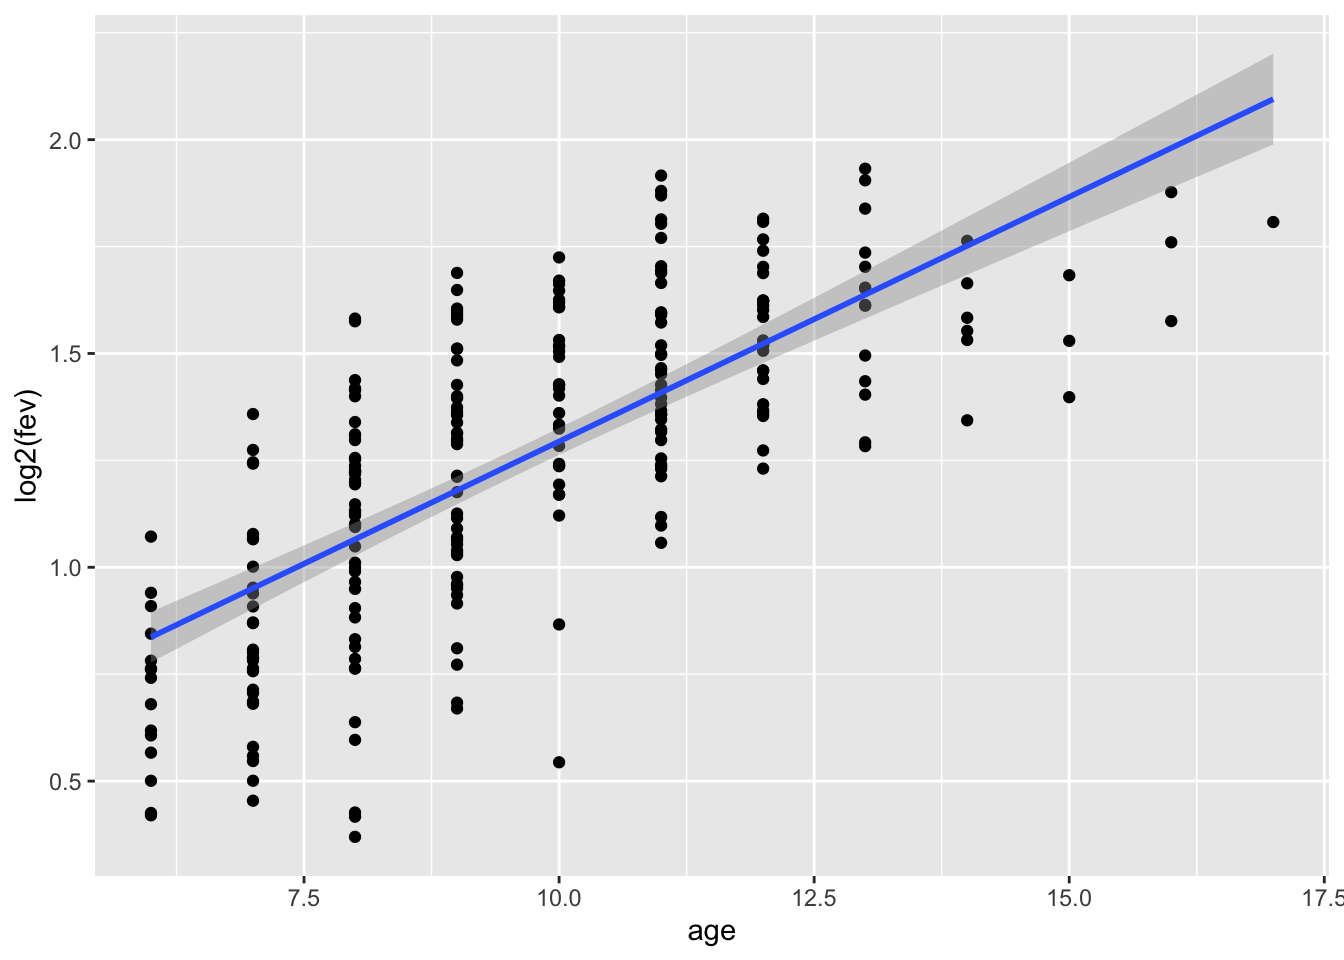
\includegraphics{introduction_files/figure-latex/unnamed-chunk-17-5.pdf}

\begin{itemize}
\tightlist
\item
  Residu plot heeft probleem aan!
\end{itemize}

\begin{Shaded}
\begin{Highlighting}[]
\NormalTok{lm3 }\OtherTok{\textless{}{-}}\NormalTok{ fev }\SpecialCharTok{\%\textgreater{}\%} 
  \FunctionTok{filter}\NormalTok{(gender}\SpecialCharTok{==}\StringTok{"f"} \SpecialCharTok{\&}\NormalTok{ smoking }\SpecialCharTok{==} \DecValTok{0}\NormalTok{) }\SpecialCharTok{\%\textgreater{}\%} 
  \FunctionTok{lm}\NormalTok{(}\FunctionTok{log2}\NormalTok{(fev)}\SpecialCharTok{\textasciitilde{}}\NormalTok{age }\SpecialCharTok{+} \FunctionTok{I}\NormalTok{(age }\SpecialCharTok{\^{}}\DecValTok{2}\NormalTok{),.)}

\FunctionTok{summary}\NormalTok{(lm3)}
\end{Highlighting}
\end{Shaded}

\begin{verbatim}
## 
## Call:
## lm(formula = log2(fev) ~ age + I(age^2), data = .)
## 
## Residuals:
##     Min      1Q  Median      3Q     Max 
## -0.8147 -0.1650  0.0153  0.1645  0.5122 
## 
## Coefficients:
##             Estimate Std. Error t value Pr(>|t|)    
## (Intercept) -1.04905    0.23698  -4.427 1.43e-05 ***
## age          0.36096    0.04725   7.639 4.57e-13 ***
## I(age^2)    -0.01202    0.00228  -5.271 2.91e-07 ***
## ---
## Signif. codes:  0 '***' 0.001 '**' 0.01 '*' 0.05 '.' 0.1 ' ' 1
## 
## Residual standard error: 0.2396 on 252 degrees of freedom
## Multiple R-squared:  0.561,  Adjusted R-squared:  0.5576 
## F-statistic:   161 on 2 and 252 DF,  p-value: < 2.2e-16
\end{verbatim}

\begin{Shaded}
\begin{Highlighting}[]
\FunctionTok{plot}\NormalTok{(lm3)}
\end{Highlighting}
\end{Shaded}

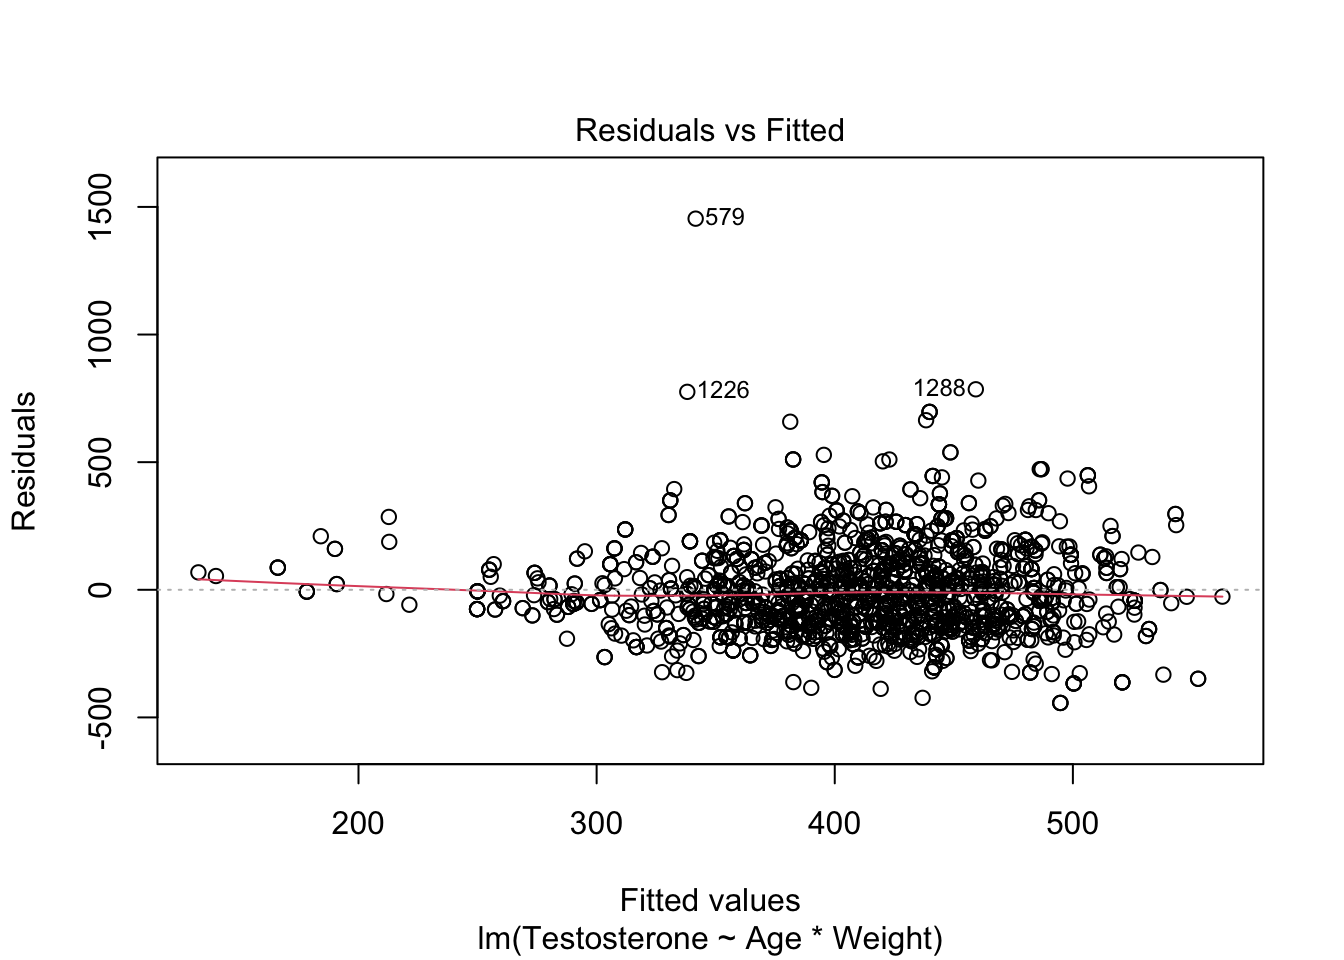
\includegraphics{introduction_files/figure-latex/unnamed-chunk-18-1.pdf}
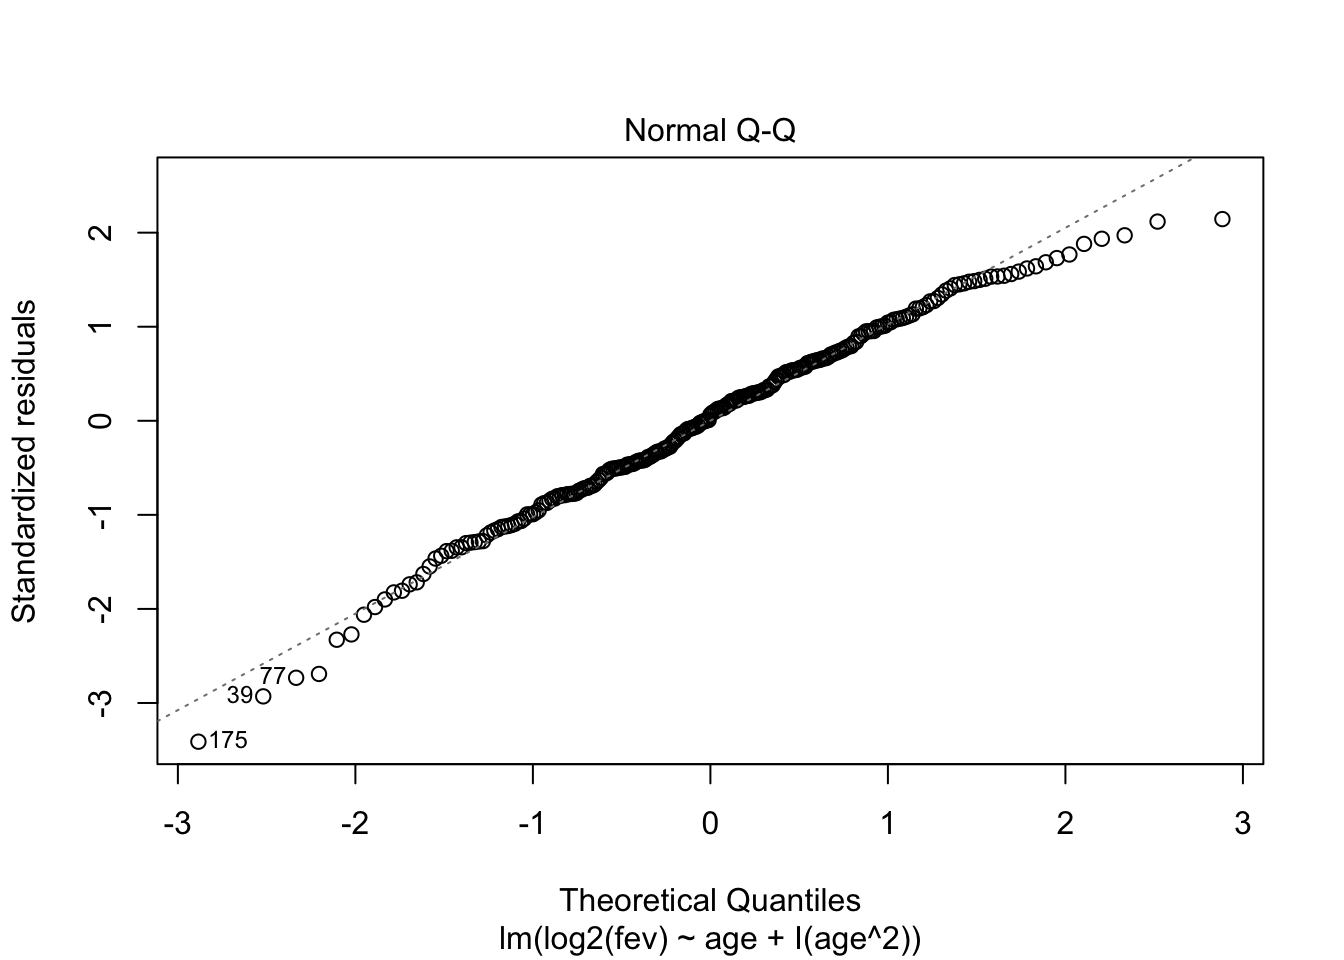
\includegraphics{introduction_files/figure-latex/unnamed-chunk-18-2.pdf}
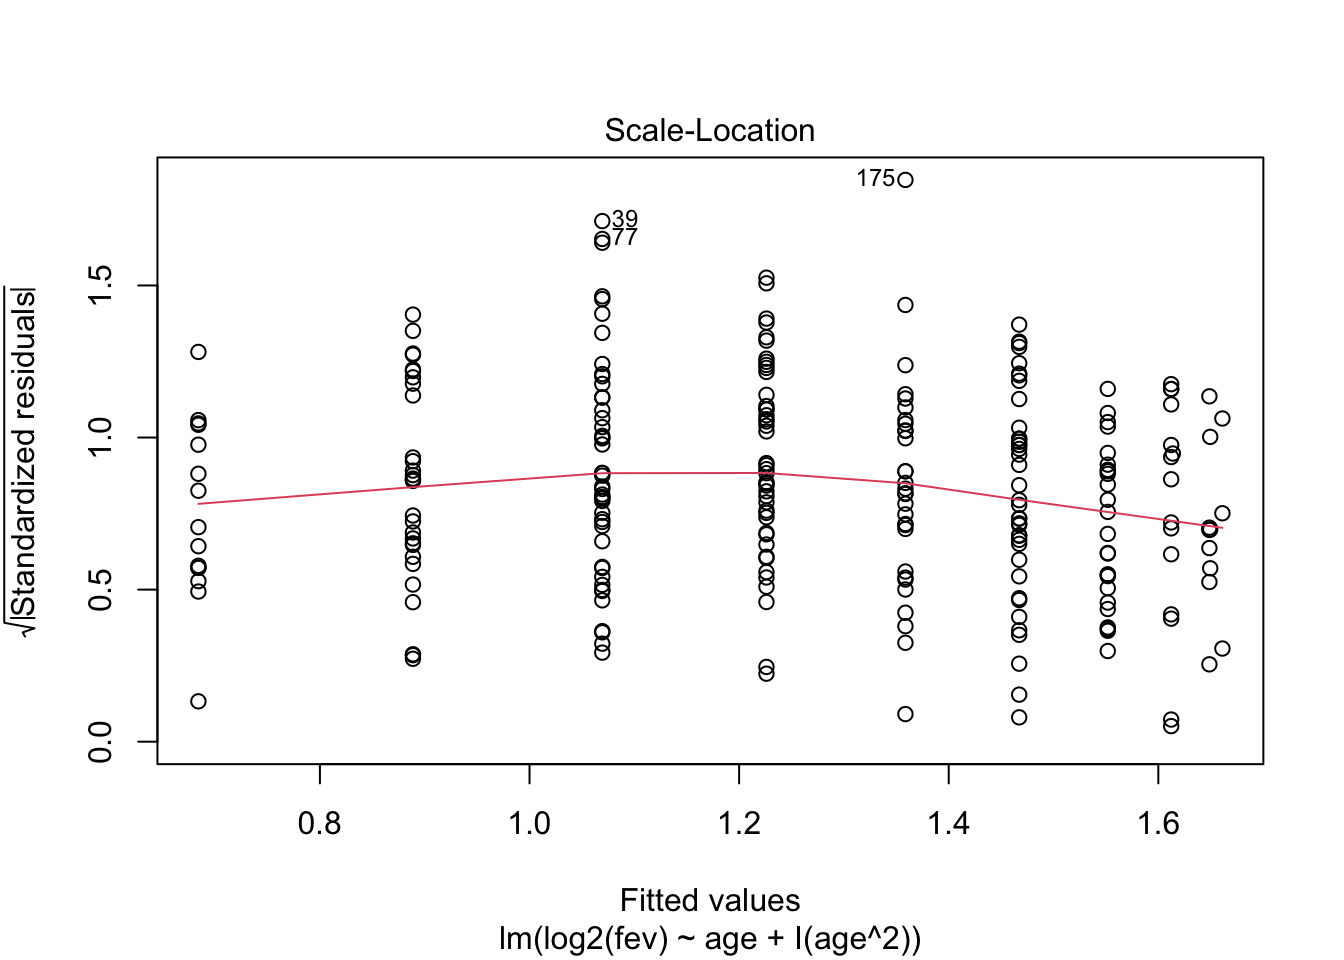
\includegraphics{introduction_files/figure-latex/unnamed-chunk-18-3.pdf}
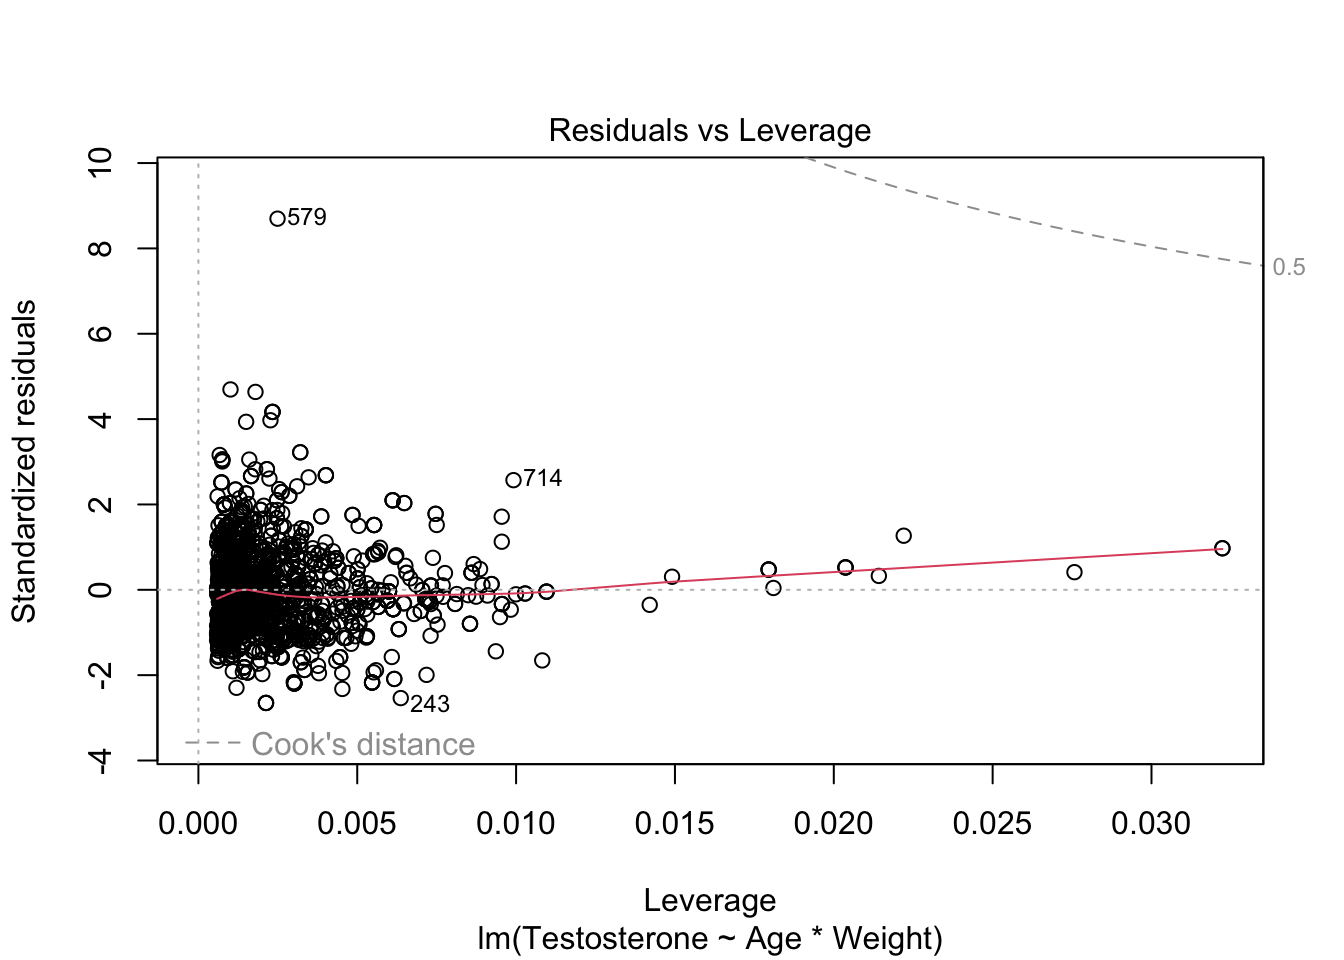
\includegraphics{introduction_files/figure-latex/unnamed-chunk-18-4.pdf}

\begin{Shaded}
\begin{Highlighting}[]
\NormalTok{fev }\SpecialCharTok{\%\textgreater{}\%} 
  \FunctionTok{ggplot}\NormalTok{(}\FunctionTok{aes}\NormalTok{(}\AttributeTok{x=}\NormalTok{age,}\AttributeTok{y=}\FunctionTok{log2}\NormalTok{(fev))) }\SpecialCharTok{+} 
  \FunctionTok{geom\_point}\NormalTok{() }\SpecialCharTok{+}
  \FunctionTok{geom\_smooth}\NormalTok{(}\AttributeTok{method =} \StringTok{"lm"}\NormalTok{, }\AttributeTok{formula =}\NormalTok{ y }\SpecialCharTok{\textasciitilde{}}\NormalTok{ x }\SpecialCharTok{+} \FunctionTok{I}\NormalTok{(x}\SpecialCharTok{\^{}}\DecValTok{2}\NormalTok{)) }\SpecialCharTok{+}
  \FunctionTok{facet\_wrap}\NormalTok{(gender }\SpecialCharTok{\textasciitilde{}}\NormalTok{ smoking)}
\end{Highlighting}
\end{Shaded}

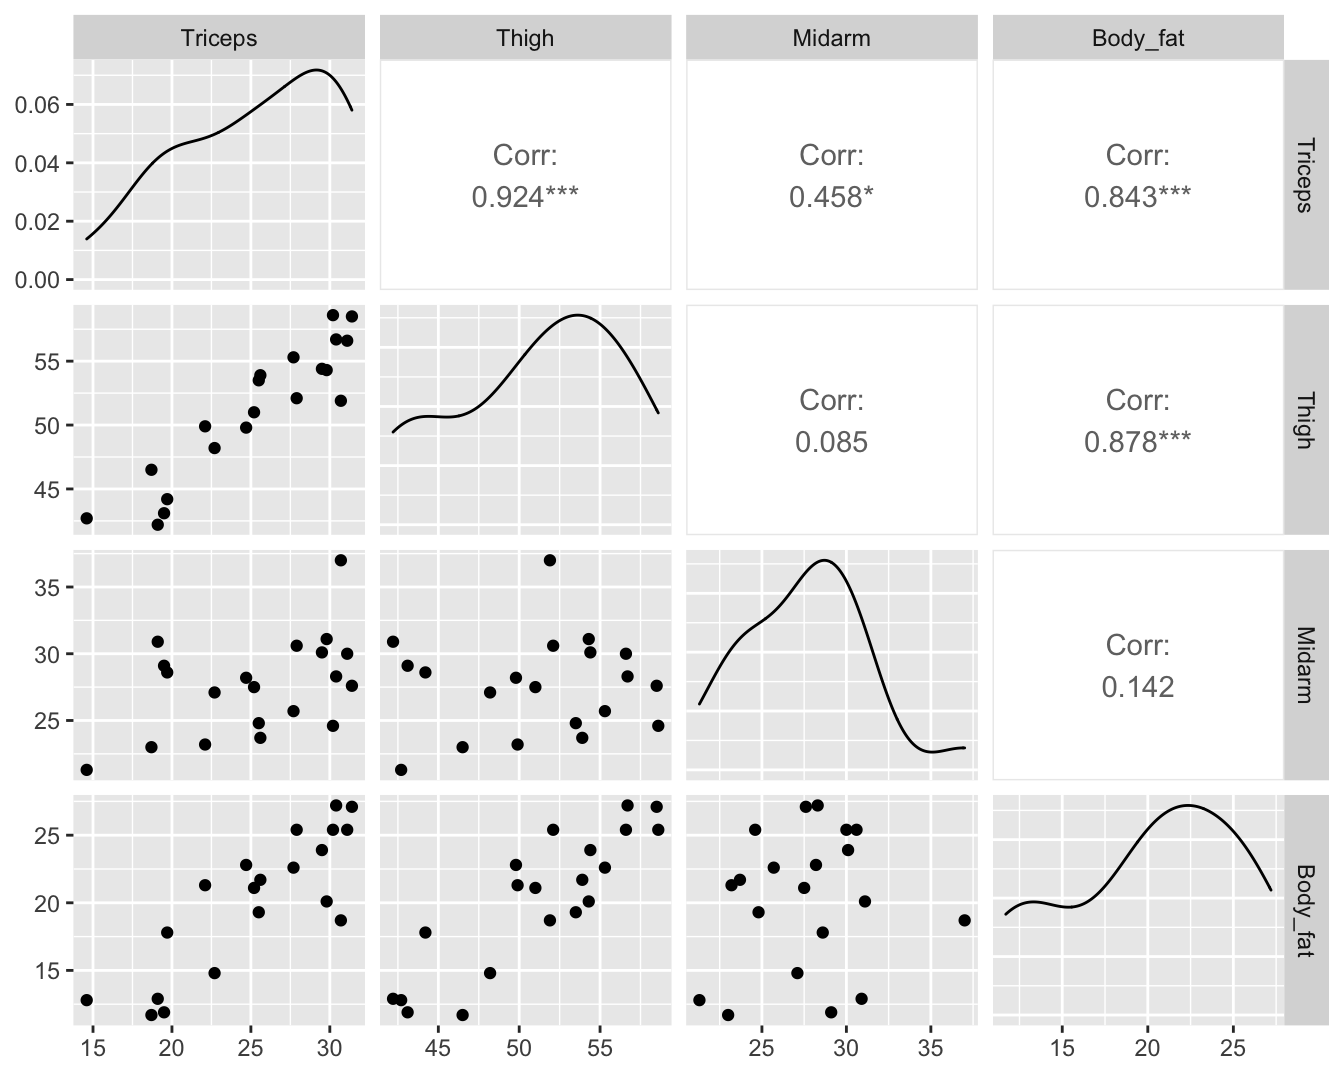
\includegraphics{introduction_files/figure-latex/unnamed-chunk-19-1.pdf}

\hypertarget{algemeen-linear-model}{%
\section{Algemeen Linear Model}\label{algemeen-linear-model}}

Hoe kunnen we meerdere factoren en continue predictoren combineren in
een lineair model?

\[
y_i= \beta_0 + \beta_S x_{i,S} + \beta_A x_{i,A}  +\epsilon_i,
\]

emt

\begin{itemize}
\tightlist
\item
  \(x_{i,S}\) een dummy variabele voor rokerstatus:
  \(x_{i,1}=\begin{cases} 0& \text{niet-roker}\\ 1& \text{roker} \end{cases}\)
\item
  \(x_{i,A}\) is de leeftijd.
\end{itemize}

\begin{center}\rule{0.5\linewidth}{0.5pt}\end{center}

\hypertarget{implementatie-in-r}{%
\subsection{Implementatie in R}\label{implementatie-in-r}}

\begin{itemize}
\tightlist
\item
  We doen dit nu enkel voor de meisjes omdat er ook effecten van
  geslacht zijn. Later leren we hoe we daarmee om kunnen gaan.
\end{itemize}

\begin{Shaded}
\begin{Highlighting}[]
\NormalTok{lmS\_age }\OtherTok{\textless{}{-}}\NormalTok{ fev }\SpecialCharTok{\%\textgreater{}\%} 
  \FunctionTok{filter}\NormalTok{(gender}\SpecialCharTok{==}\StringTok{"f"}\NormalTok{) }\SpecialCharTok{\%\textgreater{}\%}
  \FunctionTok{lm}\NormalTok{(}\FunctionTok{log2}\NormalTok{(fev)}\SpecialCharTok{\textasciitilde{}}\NormalTok{smoking }\SpecialCharTok{+}\NormalTok{ age,}\AttributeTok{data=}\NormalTok{.)}
\FunctionTok{summary}\NormalTok{(lmS\_age)}
\end{Highlighting}
\end{Shaded}

\begin{verbatim}
## 
## Call:
## lm(formula = log2(fev) ~ smoking + age, data = .)
## 
## Residuals:
##      Min       1Q   Median       3Q      Max 
## -0.74590 -0.16639  0.01665  0.19547  0.52963 
## 
## Coefficients:
##              Estimate Std. Error t value Pr(>|t|)    
## (Intercept)  0.271785   0.069410   3.916 0.000113 ***
## smoking1    -0.048477   0.051598  -0.940 0.348257    
## age          0.101810   0.006984  14.577  < 2e-16 ***
## ---
## Signif. codes:  0 '***' 0.001 '**' 0.01 '*' 0.05 '.' 0.1 ' ' 1
## 
## Residual standard error: 0.2626 on 289 degrees of freedom
## Multiple R-squared:  0.4648, Adjusted R-squared:  0.4611 
## F-statistic: 125.5 on 2 and 289 DF,  p-value: < 2.2e-16
\end{verbatim}

De parameter smoking1 krijgt nu de interpretatie van de gemiddelde log2
fold change in longinhoud tussen rokers en niet rokers na correctie voor
de leeftijd:

\begin{itemize}
\tightlist
\item
  Roker: \[E[y|\text{roker}, X_A=x] = \beta_0 + \beta_s + \beta_A x\]
\item
  Niet-roker: \[E[y|\text{niet-roker}, X_A=x] = \beta_0 + \beta_A x\]
\item
  verschil tussen roker en niet-roker van dezelfde leeftijd (\(X_A=x\)):
  \[E[y|\text{roker}, X_A=x]- E[y|\text{niet-roker}, X_A=x]=\beta_0 + \beta_s + \beta_A x- \beta_0 + \beta_A x = \beta_s\]
\end{itemize}

We weten uit de data exploratie echter dat dit nog niet het correcte
model is:

\begin{itemize}
\tightlist
\item
  Niet-lineair effect van leeftijd.
\item
  Associatie tussen FEV en rokersstatus verandert i.f.v. leeftijd,
  waarschijnlijk door associatie met hoelang al wordt gerookt. We zullen
  later zien dat dit een interactie is.
\item
  We wensen het model ook uit te breiden voor Gender.
\item
  We zien dat het niet evident is om conclusie te trekken op basis van
  observationele studies omwille van mogelijkse confounding
\item
  In de volgende lessen gaan we dieper in op het algemene lineair model
  waarin we meerdere factoren en continue variabelen kunnen combineren
  als predictoren voor het modelleren van het gemiddelde van de continue
  response variabele.
\end{itemize}

\end{document}
